\documentclass[12pt,a4paper]{report}
\usepackage[utf8]{inputenc}
\usepackage[T1]{fontenc}
\usepackage[french]{babel}
\usepackage{amsmath, amssymb, mathrsfs}
\usepackage{graphicx}
\usepackage{hyperref}
\usepackage{geometry}
\usepackage{xcolor}
\usepackage{listings}
\usepackage{booktabs}
\usepackage{fancyhdr}
\usepackage{setspace}

% Configuration de la page
\geometry{a4paper, margin=2.5cm}
\onehalfspacing % Interligne 1.5 standard pour les mémoires et thèses

% Configuration des liens
\hypersetup{
    colorlinks=true,
    linkcolor=blue,
    filecolor=magenta,      
    urlcolor=cyan,
    citecolor=black,
}

% Configuration pour le code source (si besoin)
\definecolor{codegreen}{rgb}{0,0.6,0}
\definecolor{codegray}{rgb}{0.5,0.5,0.5}
\definecolor{codepurple}{rgb}{0.58,0,0.82}
\definecolor{backcolour}{rgb}{0.95,0.95,0.92}

\lstdefinestyle{mystyle}{
    backgroundcolor=\color{backcolour},   
    commentstyle=\color{codegreen},
    keywordstyle=\color{magenta},
    numberstyle=\tiny\color{codegray},
    stringstyle=\color{codepurple},
    basicstyle=\ttfamily\footnotesize,
    breakatwhitespace=false,         
    breaklines=true,                 
    captionpos=b,                    
    keepspaces=true,                 
    numbers=left,                    
    numbersep=5pt,                  
    showspaces=false,                
    showstringspaces=false,
    showtabs=false,                  
    tabsize=2
}
\lstset{style=mystyle}

\begin{document}

% Inclusion des chapitres du rapport
\begin{titlepage}
    \centering
    \vspace*{0.5cm}
    
    
\includegraphics[width=0.4\textwidth]{images/Logo_UHIIC_0.png} \\
    \vspace{1cm}
    
    {\Large \textbf{Université Hassan II de Casablanca}} \\
    \vspace{0.2cm}
    {\large \textbf{Faculté des Sciences Juridiques, Économiques et Sociales d'Aïn Sebaâ}} \\
    \vspace{1.5cm}
    
    {\large \textbf{Rapport de Projet de Fin d'Études}} \\
    \vspace{0.5cm}
    \textit{En vue de l'obtention du diplôme de Licence Fondamentale\\ Méthodes Quantitatives Appliquées aux Sciences Sociales} \\
    
    \vspace{2cm}
    
    \hrule
    \vspace{0.5cm}
    {\huge \textbf{Gestion de Portefeuille à l'aide de \\[0.5cm] l'Intelligence Artificielle}} \\
    \vspace{0.5cm}
    \hrule
    
    \vspace{2.5cm}
    
    \begin{minipage}{0.45\textwidth}
        \begin{flushleft} \large
            \textbf{Présenté par :}\\
            Hicham \textsc{Agozol}
        \end{flushleft}
    \end{minipage}
    \hfill
    \begin{minipage}{0.45\textwidth}
        \begin{flushright} \large
            \textbf{Sous la direction de :}\\
            Mr. ALAOUI Mly Rachid
        \end{flushright>
    \end{minipage}
    
    \vfill
    
    {\large Année Universitaire 2025/2026}
    
\end{titlepage}

\chapter*{Remerciements}
\addcontentsline{toc}{chapter}{Remerciements}

Avant d'entamer le cœur de ce travail, il m'est particulièrement agréable d'exprimer ma profonde gratitude et mes sincères remerciements à toutes les personnes qui ont contribué, de près ou de loin, à l'aboutissement de ce Projet de Fin d'Études.

Je tiens tout d'abord à adresser mes remerciements les plus sincères à mon encadrant pédagogique, \textbf{Mr. ALAOUI Mly Rachid}. Ses précieux conseils, ses directives éclairées, sa disponibilité constante malgré ses nombreux engagements, ainsi que sa rigueur scientifique ont été les piliers de la réussite de ce projet. Son accompagnement bienveillant, son expertise technique et sa confiance m'ont permis de surmonter de nombreux obstacles tout au long de cette aventure. Qu'il trouve ici l'expression de mon profond respect et de ma reconnaissance la plus sincère.

Mes remerciements s'adressent également à l'ensemble du corps professoral et administratif de la Faculté des Sciences Juridiques, Économiques et Sociales d'Aïn Sebaâ (FSJESAS), Université Hassan II de Casablanca, pour la qualité de l'enseignement qui m'a été prodigué durant tout mon cursus universitaire. Leurs enseignements m'ont doté des solides compétences méthodologiques et quantitatives nécessaires pour aborder ce travail avec sérénité et ambition.

Je remercie chaleureusement les membres du jury d'avoir accepté d'évaluer ce travail de fin d'études. Leurs remarques, leurs commentaires avisés et leurs critiques constructives seront pour moi une source d'enrichissement précieuse et guideront sans doute mes futurs travaux de recherche.

Enfin, je dédie une pensée toute particulière à mes parents et à ma famille pour leur soutien moral indéfectible, leurs encouragements quotidiens et leur patience infinie durant ces mois de travail intensif. Ce modeste rapport est le fruit de leur affection inestimable et de leurs sacrifices. Que toutes les personnes qui ont contribué de près ou de loin à la réussite de ce travail trouvent ici le témoignage de ma profonde gratitude.

\newpage

\chapter*{Résumé}
\addcontentsline{toc}{chapter}{Résumé}

La gestion de portefeuille a connu une évolution majeure avec l'avènement des technologies d'Intelligence Artificielle (IA) et du Deep Learning. Ce projet de fin d'études compare l'approche d'optimisation classique de la Théorie Moderne du Portefeuille de Harry Markowitz avec des stratégies d'allocation d'actifs assistées par des modèles d'apprentissage profond. 

Nous présentons une méthodologie hybride novatrice combinant le pouvoir prédictif des réseaux de neurones récurrents de type \textbf{LSTM (Long Short-Term Memory)} avec la rigueur d'un optimiseur Moyenne-Variance. Le modèle LSTM est entraîné sur 10 ans de données historiques (2015-2024) pour prédire les rendements de grands actifs américains (Apple, Microsoft, Google, JPMorgan, Procter \& Gamble). Ces prédictions dynamiques remplacent les rendements historiques statiques dans l'algorithme d'allocation d'actifs.

Les résultats de la simulation de backtesting (2023-2024) démontrent que notre stratégie hybride surperforme significativement le marché de référence (S\&P 500) ainsi que la stratégie classique de Markowitz. Le portefeuille assisté par IA enregistre un rendement cumulé supérieur tout en maintenant un profil de risque maîtrisé, ce qui se traduit par une hausse notable du Ratio de Sharpe et une réduction des drawdowns maximaux lors des phases de correction de marché.

\textbf{Mots-clés :} Optimisation de Portefeuille, Markowitz, Intelligence Artificielle, LSTM, Deep Learning, Backtesting, Ratio de Sharpe, Marchés Financiers.

\newpage

\chapter*{Abstract}
\addcontentsline{toc}{chapter}{Abstract}

Portfolio management has undergone a major paradigm shift with the emergence of Artificial Intelligence (AI) and Deep Learning technologies. This graduation project compares the classical portfolio optimization approach of Harry Markowitz's Modern Portfolio Theory (MPT) with asset allocation strategies enhanced by deep learning models.

We present an innovative hybrid methodology combining the predictive power of Recurrent Neural Networks, specifically \textbf{LSTM (Long Short-Term Memory)} networks, with the analytical framework of a Mean-Variance optimizer. The LSTM model is trained on 10 years of historical data (2015-2024) to predict the returns of major US equities (Apple, Microsoft, Google, JPMorgan Chase, Procter \& Gamble). These dynamic predictions replace the static historical returns in the asset allocation algorithm.

The backtesting simulation results (2023-2024) demonstrate that our hybrid strategy significantly outperforms both the benchmark index (S\&P 500) and the classical Markowitz strategy. The AI-assisted portfolio achieves higher cumulative returns while maintaining a controlled risk profile, resulting in a notable increase in the Sharpe Ratio and a reduction in maximum drawdowns during market corrections.

\textbf{Keywords:} Portfolio Optimization, Markowitz, Artificial Intelligence, LSTM, Deep Learning, Backtesting, Sharpe Ratio, Financial Markets.

\newpage

% ================= TABLES DE MATIÈRES =================
\tableofcontents
\newpage
\listoffigures
\newpage
\listoftables
\newpage

% ================= LISTE DES ABRÉVIATIONS =================
\chapter*{Liste des Abréviations}
\addcontentsline{toc}{chapter}{Liste des Abréviations}

\begin{description}
    \item[ADF] Augmented Dickey-Fuller (Test de stationnarité)
    \item[API] Application Programming Interface
    \item[ARIMA] AutoRegressive Integrated Moving Average
    \item[CAPM] Capital Asset Pricing Model
    \item[CML] Capital Market Line (Droite de Marché des Capitaux)
    \item[DRL] Deep Reinforcement Learning
    \item[EMH] Efficient Market Hypothesis (Hypothèse d'Efficience du Marché)
    \item[ES] Expected Shortfall
    \item[FSJESAS] Faculté des Sciences Juridiques, Économiques et Sociales d'Aïn Sebaâ
    \item[IA] Intelligence Artificielle
    \item[LSTM] Long Short-Term Memory
    \item[MEDAF] Modèle d'Évaluation des Actifs Financiers
    \item[ML] Machine Learning
    \item[MPT] Modern Portfolio Theory (Théorie Moderne du Portefeuille)
    \item[MSE] Mean Squared Error (Erreur Quadratique Moyenne)
    \item[OPCVM] Organisme de Placement Collectif en Valeurs Mobilières
    \item[RMSE] Root Mean Square Error
    \item[RNN] Recurrent Neural Network (Réseau de neurones récurrents)
    \item[RSI] Relative Strength Index
    \item[S\&P 500] Standard \& Poor's 500
    \item[SMA] Simple Moving Average
    \item[SML] Security Market Line (Droite de Marché des Titres)
    \item[VaR] Value at Risk
\end{description}

\chapter*{Introduction Générale}
\addcontentsline{toc}{chapter}{Introduction Générale}

Depuis la nuit des temps, l'investissement financier est guidé par une quête universelle : maximiser le gain tout en minimisant la probabilité de perte. Cependant, pendant des siècles, cette gestion a reposé sur l'intuition, l'expérience empirique et parfois la spéculation pure. Ce n'est qu'au milieu du XXe siècle que la gestion de portefeuille est entrée dans l'ère scientifique avec les travaux fondateurs de Harry Markowitz en 1952. En formalisant mathématiquement le compromis entre le rendement espéré et le risque (mesuré par la variance), Markowitz a jeté les bases de la \textit{Théorie Moderne du Portefeuille} (MPT). Pour la première fois, la diversification n'était plus un simple conseil de bon sens, mais une règle quantitative rigoureuse démontrant que le risque d'un portefeuille dépend de la covariance des actifs qui le composent plutôt que de la simple somme de leurs risques individuels.

Pourtant, malgré son élégance mathématique et son adoption massive par l'industrie financière, le modèle de Markowitz repose sur des hypothèses fortes et souvent irréalistes dans la pratique. Il suppose notamment que les rendements des actifs suivent une loi normale, que les investisseurs sont strictement rationnels et que la structure statistique des rendements passés (moyennes, variances et covariances) restera stable dans le futur. Les crises financières successives de ce début de siècle (la bulle Internet en 2001, la crise des Subprimes en 2008 et le krach lié à la pandémie de COVID-19 en 2020) ont mis en lumière les limites critiques de ces modèles classiques. Sur les marchés réels, les rendements ne sont pas gaussiens ; ils affichent des « queues épaisses » (fat tails) qui augmentent la fréquence des événements extrêmes (les fameux « Cygnes Noirs » de Nassim Nicholas Taleb). De plus, l'optimiseur classique de Markowitz s'est révélé être un « amplificateur d'erreurs » : de légères modifications dans les données historiques d'entrée conduisent à des allocations de portefeuille extrêmes et impraticables.

Parallèlement, les marchés financiers ont connu une mutation technologique sans précédent. L'ère de la numérisation a entraîné une explosion du volume, de la variété et de la vitesse de propagation des données financières (le Big Data). Face à cette masse de données complexes, changeantes et souvent non-linéaires, l'analyse humaine et les outils statistiques classiques s'avèrent limités. C'est dans ce contexte que l'Intelligence Artificielle (IA) et plus spécifiquement le Machine Learning (Apprentissage Automatique) et le Deep Learning (Apprentissage Profond) se sont imposés comme des outils de rupture pour la finance quantitative.

Les réseaux de neurones artificiels, et en particulier les architectures récurrentes de type \textbf{LSTM (Long Short-Term Memory)}, ont été spécialement conçus pour modéliser des séries temporelles. Contrairement aux réseaux de neurones traditionnels, les LSTM possèdent une mémoire interne capable de capturer des dépendances temporelles à long terme et d'assimiler les dynamiques non-linéaires des marchés sans imposer d'hypothèse statistique rigide \textit{a priori} sur la distribution des prix. 

L'objet de ce Projet de Fin d'Études est de concevoir, d'implémenter et de tester une méthodologie hybride d'allocation d'actifs. Cette approche combine la puissance prédictive de l'apprentissage profond (modèle LSTM) avec le cadre d'optimisation robuste de la Théorie Moderne du Portefeuille. L'idée centrale est de substituer les rendements historiques statiques (habituellement utilisés pour estimer le vecteur des rendements espérés dans l'optimiseur de Markowitz) par des prédictions dynamiques générées par le réseau LSTM.

Pour répondre à cette problématique et évaluer l'efficacité de cette démarche, notre étude s'articulera autour de quatre chapitres principaux :

\begin{itemize}
    \item \textbf{Le Chapitre 1} posera le cadre conceptuel en présentant la structure des marchés financiers, les instruments utilisés, la modélisation mathématique classique du couple rendement-risque, ainsi que l'hypothèse d'efficience des marchés et les limites de la finance traditionnelle face au risque.
    \item \textbf{Le Chapitre 2} détaillera la transition de la théorie classique vers l'intelligence artificielle. Nous y étudierons en profondeur le modèle de Markowitz, sa formulation mathématique, la dérivation de la frontière efficiente, le MEDAF/CAPM, ainsi que les critiques et limites empiriques de ces approches classiques.
    \item \textbf{Le Chapitre 3} introduira les fondements de l'Intelligence Artificielle en finance quantitative. Nous comparerons les différents algorithmes de prédiction (Régression linéaire, ARIMA, Random Forest) et détaillerons l'architecture mathématique des réseaux de neurones récurrents LSTM. Enfin, nous décrirons le fonctionnement de notre stratégie hybride LSTM + Markowitz.
    \item \textbf{Le Chapitre 4} sera consacré à l'étude empirique. Nous y présenterons la collecte de données sur 10 ans (2015-2024) pour un portefeuille composé de grandes capitalisations américaines (AAPL, MSFT, GOOGL, JPM, PG) via l'API \texttt{yfinance}. Nous exposerons ensuite l'architecture du modèle LSTM implémenté, les résultats de son entraînement, le tracé de la frontière efficiente et, enfin, le backtesting comparatif des performances de notre stratégie face au modèle classique et à l'indice S\&P 500.
\end{itemize}

À travers ce travail, nous tenterons de déterminer si l'intégration de modèles prédictifs d'intelligence artificielle permet d'améliorer significativement le couple rendement-risque des portefeuilles réels et de surperformer les méthodes traditionnelles d'allocation d'actifs.

\chapter{Marchés Financiers et Fondements de la Gestion de Portefeuille}

\section{Introduction aux Marchés Financiers}
Les marchés financiers constituent le cœur du système économique mondial. Ils jouent un rôle fondamental d'intermédiation financière en permettant la rencontre entre deux types d'agents économiques : les agents à besoin de financement (généralement les entreprises et les États) et les agents à capacité de financement (les épargnants, les banques, les compagnies d'assurance et les fonds de pension). Cette allocation des ressources financières permet de financer les investissements productifs, de stimuler la croissance économique et d'offrir des opportunités de rendement aux investisseurs.

\section{Typologie des Actifs Financiers et Diversification}
Un portefeuille désigne l'ensemble des actifs financiers détenus par un investisseur individuel ou institutionnel. La composition d'un portefeuille peut être extrêmement variée, comprenant plusieurs classes d'actifs :

\begin{itemize}
    \item \textbf{Les Actions (Equity) :} Titres de propriété représentant une fraction du capital d'une entreprise. Ils confèrent à leur détenteur des droits politiques (droit de vote aux assemblées générales) et des droits financiers (droit de percevoir une part des bénéfices sous forme de dividendes). Les actions offrent un potentiel de rendement élevé à long terme, mais s'accompagnent d'un risque élevé en raison de la volatilité des cours et de l'absence de garantie en capital.
    \item \textbf{Les Obligations (Fixed Income) :} Titres de créance émis par des entreprises ou des entités publiques (États, collectivités) pour emprunter des capitaux sur les marchés. L'émetteur s'engage à verser régulièrement un intérêt (le coupon) et à rembourser le capital à une date d'échéance fixée (la maturité). Les obligations sont considérées comme moins risquées que les actions, mais leurs rendements sont généralement plus modestes et dépendent de la qualité de signature de l'émetteur (risque de crédit) et de l'évolution des taux d'intérêt (risque de taux).
    \item \textbf{Les Indices Boursiers :} Paniers d'actifs représentatifs d'un marché ou d'un secteur d'activité (ex : S\&P 500 pour les grandes capitalisations américaines, CAC 40 pour la France, NASDAQ pour la technologie). Ils permettent de suivre la tendance générale et de servir de référence (benchmark) pour évaluer la performance des portefeuilles gérés de manière active.
    \item \textbf{Les Organismes de Placement Collectif en Valeurs Mobilières (OPCVM) :} Véhicules d'investissement (Sicav, FCP) qui regroupent l'épargne de nombreux investisseurs pour la placer dans un portefeuille diversifié géré par des professionnels. Ils facilitent l'accès aux marchés financiers pour les particuliers.
\end{itemize}

Le concept clé sous-jacent à la gestion de portefeuille est la \textbf{diversification}. Formulé de manière populaire par l'adage « il ne faut pas mettre tous ses œufs dans le même panier », ce concept a été formalisé mathématiquement par Harry Markowitz. La diversification permet de réduire le risque global du portefeuille sans nécessairement sacrifier son rendement espéré, en exploitant le fait que les prix des différents actifs ne fluctuent pas de manière parfaitement synchronisée.

\section{Modélisation Mathématique du Rendement}
Pour analyser la performance d'un portefeuille, il convient tout d'abord de définir mathématiquement la notion de rendement. Le rendement mesure la variation relative de la valeur d'un actif sur une période donnée. Il existe deux manières principales de formuler cette variation.

\subsection{Le Rendement Discret (Simple)}
Le rendement discret ou arithmétique d'un actif $i$ sur la période allant de $t-1$ à $t$ est défini par :
\begin{equation}
    R_{i,t} = \frac{P_{i,t} - P_{i,t-1} + D_{i,t}}{P_{i,t-1}}
\end{equation}
où $P_{i,t}$ représente le prix de l'actif à l'instant $t$ et $D_{i,t}$ représente les éventuels revenus distribués (comme les dividendes) au cours de la période. Si l'on néglige les revenus distribués, la formule se simplifie :
\begin{equation}
    R_{i,t} = \frac{P_{i,t}}{P_{i,t-1}} - 1
\end{equation}
Le rendement discret d'un portefeuille composé de $n$ actifs est simplement la moyenne pondérée des rendements des actifs individuels :
\begin{equation}
    R_{p,t} = \sum_{i=1}^{n} w_i R_{i,t}
\end{equation}
où $w_i$ représente la proportion de la richesse allouée à l'actif $i$ (le poids de l'actif), avec la contrainte $\sum_{i=1}^{n} w_i = 1$.

\subsection{Le Rendement Continu (Logarithmique)}
En finance quantitative et en modélisation économétrique, on préfère souvent utiliser le rendement continu ou logarithmique, défini par :
\begin{equation}
    r_{i,t} = \ln\left(\frac{P_{i,t}}{P_{i,t-1}}\right) = \ln(P_{i,t}) - \ln(P_{i,t-1})
\end{equation}
Le rendement logarithmique présente des propriétés mathématiques particulièrement avantageuses :
\begin{enumerate}
    \item \textbf{L'additivité temporelle :} Le rendement logarithmique sur $k$ périodes est simplement la somme des rendements logarithmiques de chaque période unitaire :
    \begin{equation}
        r_{i,t}^{(k)} = \ln\left(\frac{P_{i,t}}{P_{i,t-k}}\right) = \sum_{j=0}^{k-1} r_{i,t-j}
    \end{equation}
    Cette propriété n'est pas vérifiée par les rendements discrets, car $(1 + R_{t}^{(k)}) = \prod_{j=0}^{k-1} (1 + R_{t-j})$.
    \item \textbf{La normalité statistique :} Pour de courtes périodes (comme des données journalières), les variations de prix sont petites, et le rendement continu est une très bonne approximation du rendement simple ($r_t \approx R_t$). De plus, les rendements logarithmiques se prêtent mieux à l'hypothèse de normalité en raison du théorème central limite appliqué aux sommes de variables aléatoires.
    \item \textbf{La symétrie face aux variations extrêmes :} Un rendement discret est limité inférieurement à -100\% (perte totale), mais illimité supérieurement. Le rendement logarithmique varie quant à lui sur l'intervalle $]-\infty, +\infty[$, ce qui le rend plus adapté aux modélisations statistiques basées sur des distributions symétriques.
\end{enumerate}

Toutefois, contrairement aux rendements discrets, le rendement logarithmique d'un portefeuille n'est pas la moyenne pondérée des rendements logarithmiques des actifs individuels. On doit donc souvent passer de l'un à l'autre lors des phases d'agrégation d'actifs.

\section{Modélisation Mathématique du Risque}
En finance classique, le risque est intrinsèquement lié à l'incertitude sur la valeur future d'un actif. Plus les fluctuations possibles d'un cours sont larges, plus le risque est élevé. La mesure statistique de cette dispersion est la variance ($\sigma^2$) ou l'écart-type ($\sigma$), couramment appelée \textbf{volatilité} dans le jargon financier.

Pour un actif dont les rendements historiques sur $T$ périodes sont notés $R_1, R_2, \dots, R_T$, le rendement moyen historique est calculé par :
\begin{equation}
    \bar{R} = \frac{1}{T} \sum_{t=1}^{T} R_t
\end{equation}
La variance historique, qui mesure la dispersion des rendements autour de leur moyenne, est donnée par :
\begin{equation}
    \sigma^2 = \frac{1}{T-1} \sum_{t=1}^{T} (R_t - \bar{R})^2
\end{equation}
La volatilité historique $\sigma$ est l'écart-type, soit la racine carrée de la variance :
\begin{equation}
    \sigma = \sqrt{\sigma^2}
\end{equation}
La volatilité est généralement annualisée pour permettre la comparaison entre différentes classes d'actifs ou différentes fréquences d'observation. Si l'on dispose de données journalières et que l'on suppose qu'une année compte 252 jours de bourse (trading days), la volatilité annualisée s'obtient par la formule :
\begin{equation}
    \sigma_{\text{annuel}} = \sigma_{\text{journalier}} \times \sqrt{252}
\end{equation}
De même, pour des données hebdomadaires (52 semaines) ou mensuelles (12 mois), on multipliera respectivement par $\sqrt{52}$ ou $\sqrt{12}$.

\section{L'Hypothèse d'Efficience des Marchés}
L'un des piliers de la théorie financière classique est l'Hypothèse d'Efficience des Marchés (EMH), formalisée par Eugène Fama en 1970. Selon cette théorie, un marché financier est dit efficient si les cours des titres cotés y reflètent à tout moment toute l'information disponible. Sur un tel marché, il est impossible de surperformer systématiquement le marché à risque équivalent, car les inefficiences de prix sont immédiatement arbitrées par les investisseurs rationnels.

Fama distingue trois formes d'efficience selon la nature de l'information prise en compte :

\begin{enumerate}
    \item \textbf{La forme faible (Weak form) :} Les cours passés des actifs ne contiennent aucune information utile pour prédire leurs cours futurs. Toute l'information historique est déjà intégrée dans le prix actuel. En conséquence, l'analyse technique (qui repose sur l'étude des graphiques historiques de cours) est stérile. Les cours suivent une « marche au hasard » (Random Walk) :
    \begin{equation}
        P_t = P_{t-1} + \epsilon_t
    \end{equation}
    où $\epsilon_t$ est un bruit blanc de moyenne nulle et non corrélé.
    \item \textbf{La forme semi-forte (Semi-strong form) :} Les cours intègrent non seulement l'historique des prix, mais également toute l'information publique disponible (rapports financiers des entreprises, statistiques macroéconomiques, actualités géopolitiques, etc.). Les cours s'ajustent instantanément et sans biais à l'annonce de toute nouvelle information publique. L'analyse fondamentale devient alors inefficace pour battre le marché.
    \item \textbf{La forme forte (Strong form) :} Les cours intègrent l'ensemble des informations publiques et privées (notamment les informations privilégiées ou d'initiés). Dans ce cadre extrême, même les personnes disposant d'informations confidentielles internes ne peuvent pas obtenir de rendements anormaux.
\end{enumerate}

\subsection{Anomalies de marché et Finance Comportementale}
L'hypothèse d'efficience a été vivement critiquée. L'existence d'anomalies de marché (l'effet de taille, l'effet calendrier comme « l'effet janvier », ou l'effet momentum) contredit la théorie de Fama. De plus, la finance comportementale (portée par Daniel Kahneman et Amos Tversky) a démontré que les investisseurs réels ne sont pas strictement rationnels. Ils sont soumis à des biais cognitifs (aversion à la perte, sur-confiance, comportement grégaire) qui créent des bulles spéculatives et des krachs irrationnels. Ces inefficiences locales ouvrent la voie à l'utilisation d'algorithmes avancés, comme l'Intelligence Artificielle, capables de détecter des micro-tendances comportementales complexes.

\section{Limites de la Finance Classique et Mesures de Risque Avancées}
La finance classique postule souvent que les rendements financiers suivent une loi normale (distribution gaussienne). Bien que ce postulat simplifie grandement les calculs mathématiques, il est démenti par la réalité empirique. Les rendements financiers réels présentent :
\begin{itemize}
    \item \textbf{L'asymétrie (Skewness) :} La distribution des rendements est souvent asymétrique négativement, signifiant que les baisses extrêmes sont plus fréquentes que les hausses extrêmes.
    \item \textbf{L'aplatissement (Kurtosis) élevé :} Les distributions réelles sont leptokurtiques, caractérisées par des sommets plus pointus et des « queues épaisses » (fat tails) par rapport à la loi normale. Cela implique que la probabilité d'événements extrêmes (« cygnes noirs ») est largement sous-estimée par les modèles gaussiens.
\end{itemize}

Pour pallier ces faiblesses, des mesures de risque plus adaptées ont été développées.

\subsection{La Value-at-Risk (VaR)}
La Value-at-Risk représente la perte maximale qu'un portefeuille peut subir sur un horizon temporel donné ($T$) avec un niveau de confiance fixé ($\alpha$, typiquement 95\% ou 99\%). Mathématiquement, la VaR est définie comme le quantile de la distribution des pertes du portefeuille :
\begin{equation}
    P(\text{Perte} > \text{VaR}_{\alpha}) = 1 - \alpha
\end{equation}
Bien que très populaire et réglementée (notamment dans les accords bancaires de Bâle), la VaR présente deux limites majeures : elle ne dit rien sur l'ampleur des pertes au-delà du seuil de confiance, et elle n'est pas mathématiquement subadditive (le risque d'un portefeuille fusionné peut être supérieur à la somme des risques individuels, contredisant le principe de diversification).

\subsection{L'Expected Shortfall (ES)}
L'Expected Shortfall (ou VaR conditionnelle) mesure l'espérance de la perte sachant que celle-ci dépasse le seuil de la VaR. C'est une mesure cohérente de risque qui résout les faiblesses de la VaR :
\begin{equation}
    \text{ES}_{\alpha} = E[\text{Perte} \mid \text{Perte} > \text{VaR}_{\alpha}]
\end{equation}
L'Expected Shortfall est particulièrement sensible aux « queues épaisses » et donne une image beaucoup plus réaliste du risque de perte extrême sur les marchés financiers modernes.

\chapter{La Théorie Moderne du Portefeuille et le Modèle d'Optimisation Classique}

\section{Le Modèle de Markowitz (1952)}
La Théorie Moderne du Portefeuille (MPT), introduite par Harry Markowitz dans son article fondateur de 1952 intitulé \textit{« Portfolio Selection »}, repose sur l'idée que le choix d'un investissement ne doit pas se faire sur la base de son seul rendement espéré, mais sur le couple rendement-risque. Dans ce cadre, le risque est mesuré par la variance des rendements. 

Markowitz a démontré que le risque d'un portefeuille d'actifs financiers est généralement inférieur à la somme pondérée des risques de chaque actif pris individuellement. Cet effet bénéfique s'explique par la corrélation imparfaite entre les rendements des différents actifs.

\subsection{Formalisation Mathématique d'un Portefeuille}
Soit un univers composé de $n$ actifs financiers. Le rendement espéré de chaque actif $i$ est noté $E(R_i)$ et sa volatilité (écart-type) est notée $\sigma_i$.
On définit les variables de décision suivantes :
\begin{equation}
    w = \begin{pmatrix} w_1 \\ w_2 \\ \vdots \\ w_n \end{pmatrix}
\end{equation}
où $w_i$ représente la proportion du capital total investi dans l'actif $i$. Ces poids doivent satisfaire la contrainte budgétaire :
\begin{equation}
    \sum_{i=1}^{n} w_i = 1 \quad \text{soit} \quad w^T \mathbf{1} = 1
\end{equation}
où $\mathbf{1}$ est un vecteur colonne de dimensions $n \times 1$ dont toutes les composantes sont égales à 1.

\subsection{Rendement Espéré du Portefeuille}
Le rendement espéré du portefeuille $E(R_p)$ est la combinaison linéaire des rendements espérés des actifs individuels :
\begin{equation}
    E(R_p) = \sum_{i=1}^{n} w_i E(R_i) = w^T E(R)
\end{equation}
où $E(R) = \begin{pmatrix} E(R_1) & E(R_2) & \dots & E(R_n) \end{pmatrix}^T$ est le vecteur des rendements espérés des actifs.

\subsection{Risque (Variance) du Portefeuille}
La variance des rendements du portefeuille, notée $\sigma_p^2$, dépend non seulement de la variance des actifs individuels mais aussi de leurs covariances :
\begin{equation}
    \sigma_p^2 = \sum_{i=1}^{n} \sum_{j=1}^{n} w_i w_j \sigma_{ij} = w^T \Sigma w
\end{equation}
où $\sigma_{ij}$ représente la covariance entre le rendement de l'actif $i$ et celui de l'actif $j$ (avec $\sigma_{ii} = \sigma_i^2$ la variance de l'actif $i$), et $\Sigma$ désigne la matrice de variance-covariance de dimensions $n \times n$ :
\begin{equation}
    \Sigma = \begin{pmatrix}
        \sigma_1^2 & \sigma_{12} & \dots & \sigma_{1n} \\
        \sigma_{21} & \sigma_2^2 & \dots & \sigma_{2n} \\
        \vdots & \vdots & \ddots & \vdots \\
        \sigma_{n1} & \sigma_{n2} & \dots & \sigma_n^2
    \end{pmatrix}
\end{equation}
La covariance peut également être exprimée en utilisant le coefficient de corrélation linéaire de Pearson $\rho_{ij}$ :
\begin{equation}
    \sigma_{ij} = \rho_{ij} \sigma_i \sigma_j
\end{equation}
avec $-1 \le \rho_{ij} \le 1$. C'est ce coefficient de corrélation $\rho_{ij}$ qui détermine l'efficacité de la diversification :
\begin{itemize}
    \item Si $\rho_{ij} = 1$ : Les actifs sont parfaitement corrélés positivement. Il n'y a aucun effet de diversification. Le risque du portefeuille est la moyenne pondérée des risques individuels.
    \item Si $\rho_{ij} < 1$ : La volatilité du portefeuille est strictement inférieure à la moyenne pondérée des volatilités individuelles. Le risque global diminue.
    \item Si $\rho_{ij} = -1$ : Les actifs sont parfaitement corrélés négativement. Il est théoriquement possible de construire un portefeuille à risque nul en combinant ces deux actifs.
\end{itemize}

\section{Le Problème d'Optimisation et Dérivation Mathématique}
L'investisseur de Markowitz est caractérisé par son aversion au risque et sa rationalité. Pour construire son portefeuille, il est confronté à un double objectif contradictoire : maximiser son rendement attendu pour un niveau de risque donné, ou minimiser son risque pour un rendement attendu cible.

Mathématiquement, le problème de minimisation de la variance pour un rendement cible $R^*$ s'écrit sous la forme suivante :
\begin{equation}
    \begin{aligned}
        & \min_{w} \frac{1}{2} w^T \Sigma w \\
        & \text{sous les contraintes :} \\
        & w^T E(R) = R^* \\
        & w^T \mathbf{1} = 1
    \end{aligned}
\end{equation}
Le facteur $\frac{1}{2}$ devant la variance est introduit pour simplifier les calculs de dérivation.

\subsection{Résolution par la Méthode des Multiplicateurs de Lagrange}
Pour résoudre ce problème d'optimisation quadratique sous contraintes d'égalité, on introduit le Lagrangien $\mathcal{L}$ :
\begin{equation}
    \mathcal{L}(w, \lambda_1, \lambda_2) = \frac{1}{2} w^T \Sigma w - \lambda_1 (w^T E(R) - R^*) - \lambda_2 (w^T \mathbf{1} - 1)
\end{equation}
où $\lambda_1$ et $\lambda_2$ sont les multiplicateurs de Lagrange associés respectivement à la contrainte de rendement cible et à la contrainte budgétaire.

Les conditions de premier ordre (CPO) s'obtiennent en annulant les dérivées partielles du Lagrangien par rapport aux poids $w$ et aux multiplicateurs :
\begin{align}
    \frac{\partial \mathcal{L}}{\partial w} = \Sigma w - \lambda_1 E(R) - \lambda_2 \mathbf{1} = 0 \\
    \frac{\partial \mathcal{L}}{\partial \lambda_1} = w^T E(R) - R^* = 0 \\
    \frac{\partial \mathcal{L}}{\partial \lambda_2} = w^T \mathbf{1} - 1 = 0
\end{align}

De l'équation (2.11), on exprime le vecteur de poids optimal $w^*$ en multipliant par l'inverse de la matrice de covariance $\Sigma^{-1}$ (en supposant que la matrice est définie positive et donc inversible) :
\begin{equation}
    w^* = \lambda_1 \Sigma^{-1} E(R) + \lambda_2 \Sigma^{-1} \mathbf{1}
\end{equation}
En injectant cette expression de $w^*$ dans les équations de contraintes (2.12) et (2.13), on obtient un système d'équations linéaires à deux inconnues ($\lambda_1$ et $\lambda_2$) :
\begin{align}
    \lambda_1 E(R)^T \Sigma^{-1} E(R) + \lambda_2 E(R)^T \Sigma^{-1} \mathbf{1} = R^* \\
    \lambda_1 \mathbf{1}^T \Sigma^{-1} E(R) + \lambda_2 \mathbf{1}^T \Sigma^{-1} \mathbf{1} = 1
\end{align}

Pour simplifier l'écriture, on définit les constantes statistiques classiques suivantes :
\begin{align}
    A &= E(R)^T \Sigma^{-1} E(R) \\
    B &= E(R)^T \Sigma^{-1} \mathbf{1} = \mathbf{1}^T \Sigma^{-1} E(R) \\
    C &= \mathbf{1}^T \Sigma^{-1} \mathbf{1}
\end{align}
Le système s'écrit alors :
\begin{align}
    A \lambda_1 + B \lambda_2 = R^* \\
    B \lambda_1 + C \lambda_2 = 1
\end{align}
Le déterminant de ce système est $D = AC - B^2$. En résolvant pour $\lambda_1$ et $\lambda_2$, on trouve :
\begin{align}
    \lambda_1 &= \frac{C R^* - B}{AC - B^2} \\
    \lambda_2 &= \frac{A - B R^*}{AC - B^2}
\end{align
En substituant ces multiplicateurs dans l'équation (2.14), on obtient l'expression analytique finale des poids optimaux pour un rendement cible donné :
\begin{equation}
    w^* = \frac{C R^* - B}{AC - B^2} \Sigma^{-1} E(R) + \frac{A - B R^*}{AC - B^2} \Sigma^{-1} \mathbf{1}
\end{equation}

\section{La Frontière Efficiente}
En faisant varier le rendement cible $R^*$, on trace une courbe dans le plan (Risque, Rendement) reliant l'ensemble des portefeuilles minimisant la variance. Cette enveloppe est une hyperbole. 

La partie supérieure de cette hyperbole (située au-dessus du portefeuille de variance minimale globale, appelé \textit{Global Minimum Variance Portfolio} ou GMVP) est appelée la \textbf{Frontière Efficiente}. Tout portefeuille situé sur cette frontière offre le rendement maximal pour un niveau de risque donné. Un investisseur rationnel choisira exclusivement son allocation parmi les portefeuilles de cette frontière, le choix final dépendant de son degré personnel d'aversion au risque.

\section{Le Modèle d'Évaluation des Actifs Financiers (MEDAF)}
Développé par William Sharpe (1964), John Lintner (1965) et Jan Mossin (1966), le Modèle d'Évaluation des Actifs Financiers (MEDAF, ou CAPM en anglais) prolonge le travail de Markowitz en y introduisant l'existence d'un \textbf{actif sans risque} (comme les bons du Trésor à court terme d'un État stable).

\subsection{La Droite de Marché des Capitaux (CML)}
En combinant l'actif sans risque (de rendement certain $R_f$ et de volatilité nulle) avec le portefeuille d'actifs risqués, la frontière efficiente n'est plus une hyperbole mais devient une droite tangente à l'hyperbole de Markowitz. Cette droite est appelée la \textbf{Droite de Marché des Capitaux} (Capital Market Line - CML).

Le point de tangence correspond au \textbf{Portefeuille de Marché} ($M$), composé de tous les actifs risqués disponibles pondérés par leur capitalisation boursière. La formule de la CML s'écrit :
\begin{equation}
    E(R_p) = R_f + \left[ \frac{E(R_m) - R_f}{\sigma_m} \right] \sigma_p
\end{equation
où $E(R_m)$ et $\sigma_m$ désignent respectivement le rendement espéré et la volatilité du portefeuille de marché. Le terme entre crochets représente le prix du risque sur le marché.

\subsection{Le Beta et la Droite de Marché des Titres (SML)}
À l'équilibre du marché, le MEDAF stipule que le rendement espéré de n'importe quel actif individuel $i$ est lié linéairement à son risque systématique, mesuré par le coefficient Beta ($\beta_i$) :
\begin{equation}
    E(R_i) = R_f + \beta_i (E(R_m) - R_f)
\end{equation}
Le Beta de l'actif $i$ mesure la sensibilité de son rendement par rapport à celui du portefeuille de marché :
\begin{equation}
    \beta_i = \frac{\text{Cov}(R_i, R_m)}{\text{Var}(R_m)}
\end{equation}
Le risque d'un actif individuel est ainsi scindé en deux composantes :
\begin{enumerate}
    \item \textbf{Le risque spécifique (ou idiosyncratique) :} Propre à l'entreprise émettrice. Ce risque peut être entièrement éliminé par une diversification adéquate.
    \item \textbf{Le risque systématique (ou risque de marché) :} Lié aux fluctuations globales de l'économie. Ce risque ne peut pas être diversifié. Le MEDAF indique que le marché ne rémunère que la prise de risque systématique.
\end{enumerate}

La représentation graphique de la relation du MEDAF est la \textbf{Droite de Marché des Titres} (Security Market Line - SML). Un actif sous-évalué se situera au-dessus de la SML (son rendement espéré est anormalement élevé par rapport à son risque), tandis qu'un actif surévalué se situera au-dessous.

\subsection{Le Ratio de Sharpe}
Dérivé du MEDAF, le Ratio de Sharpe ($S$) mesure la performance d'un portefeuille ajustée du risque. Il se définit comme l'excédent de rendement par rapport au taux sans risque divisé par la volatilité globale du portefeuille :
\begin{equation}
    S = \frac{E(R_p) - R_f}{\sigma_p}
\end{equation}
Un ratio supérieur à 0 indique que le portefeuille surperforme l'actif sans risque. Un ratio supérieur à 1 est considéré comme très performant sur les marchés d'actions. L'objectif de l'optimisation est généralement de maximiser ce ratio (Portefeuille de Sharpe Maximum).

\section{Limites de la Théorie Classique}
Malgré sa puissance théorique, l'optimisation classique de Markowitz présente des limites majeures qui entravent son utilisation brute sur les marchés financiers réels :

\begin{enumerate}
    \item \textbf{Le phénomène « Garbage In, Garbage Out » (GIGO) :} L'optimiseur de Markowitz est extrêmement sensible aux paramètres d'entrée (vecteur des rendements espérés et matrice de covariance). Une erreur d'estimation de 1\% sur le rendement attendu d'un actif peut modifier du tout au tout les poids optimaux calculés, menant à des allocations irréalistes ou à des positions excessivement concentrées.
    \item \textbf{Instabilité de la matrice de covariance :} L'estimation de la matrice de covariance par des séries historiques est instable, en particulier lorsque le nombre d'actifs $n$ est grand par rapport au nombre d'observations historiques $T$ (problème de dimensionalité).
    \item \textbf{Non-normalité des rendements :} La MPT suppose des rendements gaussiens et n'évalue le risque que par la variance. Or, la variance traite de manière symétrique les écarts positifs (gains) et négatifs (pertes), ce qui ne correspond pas aux préférences des investisseurs réels qui ne craignent que le risque de baisse.
\end{enumerate}

Pour surmonter ces faiblesses, plusieurs approches de régularisation ont été introduites, comme le modèle de Black-Litterman (qui intègre les opinions des gérants). L'intégration de modèles d'apprentissage automatique (Machine Learning / Deep Learning) offre une alternative moderne prometteuse en remplaçant l'estimation statistique historique par des prédictions intelligentes et non-linéaires.

\chapter{Intelligence Artificielle et Deep Learning pour la Prévision Financière}

\section{Introduction à l'Intelligence Artificielle en Finance}
L'Intelligence Artificielle (IA) désigne l'ensemble des théories et techniques mises en œuvre en vue de réaliser des machines capables de simuler l'intelligence humaine. Dans le secteur financier, l'IA s'est d'abord développée sous forme de systèmes experts basés sur des règles métier avant de connaître une révolution avec l'avènement du Machine Learning (Apprentissage Automatique) et du Deep Learning (Apprentissage Profond).

Contrairement à la programmation classique où l'ingénieur écrit les règles de calcul pour obtenir un résultat à partir de données, le Machine Learning inverse ce paradigme : l'algorithme ingère des données et les résultats attendus pour apprendre de manière autonome les règles sous-jacentes.

\section{Comparaison des Algorithmes de Prédiction}
L'analyse prédictive des séries temporelles financières peut être réalisée par plusieurs classes de modèles, dont il convient de comprendre les spécificités et les limites.

\subsection{Modèles Statistiques Classiques : ARIMA}
Les modèles autorégressifs intégrés de moyenne mobile (ARIMA) constituent le standard de la statistique classique pour l'analyse des séries temporelles. Un modèle $ARIMA(p, d, q)$ modélise une variable en fonction de ses propres valeurs passées ($p$ termes autorégressifs) et des erreurs de prédiction passées ($q$ termes de moyenne mobile), après avoir stationnarisé la série par différenciation ($d$).
Bien que robustes et faciles à interpréter, les modèles ARIMA souffrent de limites sévères en finance :
\begin{itemize}
    \item Ils supposent des relations strictement linéaires entre les variables.
    \item Ils requièrent des séries temporelles stationnaires en moyenne et en variance.
    \item Ils peinent à s'adapter aux changements structurels de régime sur les marchés financiers.
\end{itemize}

\subsection{Algorithmes de Machine Learning : Random Forest}
Le Random Forest (Forêt Aléatoire) est un algorithme d'apprentissage supervisé basé sur l'assemblage de multiples arbres de décision (Bagging). En combinant les prédictions de centaines d'arbres entraînés sur des sous-ensembles aléatoires de données, Random Forest réduit le risque de sur-apprentissage (overfitting) et s'avère excellent pour capturer des relations non-linéaires complexes.
Néanmoins, son principal inconvénient pour les séries temporelles est qu'il ne prend pas nativement en compte l'ordre chronologique des observations. Les données doivent être transformées sous forme de variables décalées (lags), et le modèle traite chaque ligne de données de manière indépendante, sans mémoire interne des séquences passées.

\subsection{Apprentissage Profond et Réseaux de Neurones Récurrents}
Le Deep Learning utilise des réseaux de neurones artificiels profonds (comportant de nombreuses couches cachées) pour extraire automatiquement des représentations complexes à partir des données brutes. 
Pour traiter les données séquentielles (comme les cours de bourse), les réseaux de neurones classiques (Feedforward) sont inadaptés car ils supposent que les entrées sont indépendantes les unes des autres. Les **Réseaux de Neurones Récurrents (RNN)** corrigent cette lacune en introduisant des boucles de rétroaction. L'information circule d'un pas de temps à un autre grâce à un état caché qui fait office de mémoire interne.

Cependant, les RNN classiques souffrent d'un problème mathématique majeur lors de leur entraînement par rétropropagation du gradient à travers le temps : le phénomène de \textbf{disparition du gradient} (vanishing gradient) ou d'\textbf{explosion du gradient}. Lorsque la séquence temporelle est longue, le gradient (qui sert à mettre à jour les poids du réseau) est multiplié à chaque pas de temps par des valeurs proches de zéro (ou supérieures à un), ce qui le fait tendre vers zéro (ou vers l'infini). En conséquence, le réseau devient incapable de retenir des dépendances temporelles à long terme.

\section{Architecture des Réseaux LSTM}
Pour résoudre le problème de disparition du gradient, Sepp Hochreiter et Jürgen Schmidhuber ont introduit en 1997 l'architecture \textbf{LSTM (Long Short-Term Memory)}. Le réseau LSTM remplace les neurones classiques des couches cachées par des cellules de mémoire complexes (LSTM memory cells). 

L'élément central d'une cellule LSTM est son **état de cellule** (cell state), représenté par $C_t$, qui traverse toute la chaîne récurrente avec seulement quelques interactions linéaires mineures, agissant comme une « autoroute de l'information ». La régulation des flux d'information au sein de la cellule s'effectue via trois portes mathématiques (gates) : la porte d'oubli, la porte d'entrée et la porte de sortie.

\begin{figure}[h]
    \centering
    % Représentation schématique conceptuelle d'une cellule LSTM
    \fbox{
        \begin{minipage}{0.85\textwidth}
            \centering
            \vspace{0.2cm}
            \textbf{Schéma Mathématique d'une Cellule LSTM} \\
            \vspace{0.4cm}
            Entrées : $x_t$ (nouvelle donnée), $h_{t-1}$ (état caché précédent), $C_{t-1}$ (état de cellule précédent) \\
            $\Downarrow$ \\
            Porte d'oubli ($f_t$) $\rightarrow$ Décide quoi oublier de $C_{t-1}$ \\
            Porte d'entrée ($i_t$ \& $\tilde{C}_t$) $\rightarrow$ Décide quelles nouvelles informations stocker dans $C_t$ \\
            Mise à jour : $C_t = f_t * C_{t-1} + i_t * \tilde{C}_t$ \\
            Porte de sortie ($o_t$ \& $h_t$) $\rightarrow$ Filtre l'information pour l'état caché de sortie $h_t$ \\
            $\Downarrow$ \\
            Sorties : $h_t$ (état caché actuel), $C_t$ (état de cellule actuel)
            \vspace{0.2cm}
        \end{minipage}
    }
    \caption{Flux de traitement et portes au sein d'une cellule LSTM}
    \label{fig:lstm_cell}
\end{figure}

Voici la description mathématique pas-à-pas du traitement au sein d'une cellule LSTM à l'instant $t$ :

\subsection{1. La Porte d'Oubli (Forget Gate)}
Cette porte détermine quelle quantité de l'information passée doit être conservée ou jetée. Elle prend en entrée l'état caché précédent $h_{t-1}$ et le vecteur d'entrée actuel $x_t$, et applique une fonction d'activation sigmoïde ($\sigma$) :
\begin{equation}
    f_t = \sigma(W_f \cdot [h_{t-1}, x_t] + b_f)
\end{equation}
où $W_f$ représente la matrice des poids de la porte d'oubli, $b_f$ le vecteur de biais, et $[h_{t-1}, x_t]$ la concaténation de l'état caché précédent et de l'entrée. La fonction sigmoïde renvoie des valeurs comprises entre 0 (oublier complètement) et 1 (conserver entièrement).

\subsection{2. La Porte d'Entrée (Input Gate)}
Cette étape décide quelles nouvelles informations seront stockées dans l'état de cellule. Elle se compose de deux parties :
* La fonction sigmoïde de la porte d'entrée ($i_t$) décide quelles valeurs seront mises à jour :
\begin{equation}
    i_t = \sigma(W_i \cdot [h_{t-1}, x_t] + b_i)
\end{equation}
* Une couche tangente hyperbolique ($\tanh$) crée un vecteur de nouvelles valeurs candidates ($\tilde{C}_t$) qui pourraient être ajoutées à l'état de cellule :
\begin{equation}
    \tilde{C}_t = \tanh(W_c \cdot [h_{t-1}, x_t] + b_c)
\end{equation}

\subsection{3. Mise à jour de l'État de Cellule}
L'ancien état de cellule $C_{t-1}$ est mis à jour pour devenir le nouvel état $C_t$. On multiplie l'ancien état par la porte d'oubli $f_t$, puis on ajoute les nouvelles informations candidates pondérées par la porte d'entrée $i_t$ :
\begin{equation}
    C_t = f_t * C_{t-1} + i_t * \tilde{C}_t
\end{equation}
où $*$ désigne le produit de Hadamard (produit matriciel terme à terme).

\subsection{4. La Porte de Sortie (Output Gate)}
Cette porte détermine la valeur de l'état caché $h_t$ qui sera envoyé en sortie de la cellule et servira d'entrée au pas de temps suivant :
* On applique d'abord une fonction sigmoïde sur les entrées pour décider quelles parties de l'état de cellule vont être extraites :
\begin{equation}
    o_t = \sigma(W_o \cdot [h_{t-1}, x_t] + b_o)
\end{equation}
* On multiplie ensuite l'état de cellule $C_t$ (passé par la fonction non-linéaire $\tanh$) par la porte de sortie $o_t$ pour obtenir le nouvel état caché :
\begin{equation}
    h_t = o_t * \tanh(C_t)
\end{equation}

Grâce à ce mécanisme de portes, le réseau LSTM peut apprendre à retenir des motifs temporels complexes sur de très longues séquences (plusieurs dizaines de pas de temps), ce qui en fait l'outil idéal pour analyser des cours financiers qui dépendent d'historiques de prix de plusieurs semaines.

\section{Stratégie Hybride LSTM + Markowitz}
La stratégie d'optimisation classique de Markowitz présente une faiblesse majeure : elle utilise des rendements historiques moyens pour estimer les rendements futurs espérés $E(R_i)$. Cette approche rétrospective présuppose implicitement que le futur sera identique au passé récent.

Notre **stratégie hybride** propose une approche prospective (forward-looking) en deux étapes :
\begin{enumerate}
    \item **Phase Prédictive (IA) :** Pour chaque actif du portefeuille, un réseau LSTM est entraîné sur l'historique des cours. Le modèle prend en entrée les rendements et indicateurs techniques récents (ex : les 10 derniers jours de bourse) et génère une prédiction pour le rendement du jour suivant :
    \begin{equation}
        \hat{R}_{i,t+1} = \text{LSTM}_i(R_{i,t}, R_{i,t-1}, \dots, R_{i,t-9}, \text{Features}_t)
    \end{equation}
    Le vecteur des prédictions $\hat{R}_{t+1} = \begin{pmatrix} \hat{R}_{1,t+1} & \dots & \hat{R}_{n,t+1} \end{pmatrix}^T$ constitue notre estimation prospective des rendements espérés.
    \item **Phase d'Allocation (MPT) :** Au lieu d'injecter la moyenne historique $E(R)$ dans le problème d'optimisation (2.8), nous y injectons les rendements prédits par l'IA $\hat{R}$. L'optimiseur résout alors le problème de maximisation du ratio de Sharpe ou de minimisation du risque sous contrainte de ce rendement attendu prédit :
    \begin{equation}
        \max_{w_t} \frac{w_t^T \hat{R}_{t+1} - R_f}{\sqrt{w_t^T \Sigma w_t}}
    \end{equation}
    La matrice de covariance $\Sigma$ est quant à elle estimée de manière classique (ou régularisée) sur la base des rendements historiques, car la structure de corrélation entre les actifs est généralement plus stable dans le temps que le sens de variation des prix.
\end{enumerate}

Cette approche hybride associe le meilleur des deux mondes : la puissance prédictive non-linéaire de l'Intelligence Artificielle pour capter les tendances des prix, et la rigueur de la théorie moderne du portefeuille pour structurer le contrôle du risque global via la matrice de corrélation.

\chapter{Étude Empirique et Analyses Comparatives des Résultats}

\section{Présentation du Dataset et Collecte des Données}
Pour valider empiriquement notre méthodologie hybride, nous avons sélectionné un portefeuille d'investissement diversifié composé de cinq grandes capitalisations boursières américaines, cotées sur l'indice S\&P 500. Ces actifs ont été choisis pour représenter différents secteurs de l'économie globale et pour leur forte liquidité :
\begin{itemize}
    \item \textbf{Apple Inc. (AAPL) :} Secteur de la technologie grand public et du matériel informatique.
    \item \textbf{Microsoft Corp. (MSFT) :} Secteur du logiciel, du cloud computing et de l'infrastructure technologique.
    \item \textbf{Alphabet Inc. (GOOGL) :} Secteur des services internet, de la publicité numérique et des technologies d'IA.
    \item \textbf{JPMorgan Chase \& Co. (JPM) :} Secteur des services financiers et de la banque d'investissement.
    \item \textbf{The Procter \& Gamble Company (PG) :} Secteur des biens de consommation de base (défensif).
\end{itemize}

L'indice S\&P 500 (\texttt{\textasciicircum GSPC}) est utilisé comme benchmark de marché (portefeuille de référence). Les données de prix de clôture quotidiens ajustés ont été extraites via l'API financière Yahoo Finance (\texttt{yfinance}). 

La période d'étude s'étend du \textbf{1er Janvier 2015 au 31 Décembre 2024}, soit un total de 10 années de cotations journalières. Cette longue période d'analyse est particulièrement intéressante car elle intègre des régimes de marché variés :
* Une phase de hausse prolongée (Bull Market) entre 2015 et 2019.
* Le choc systémique extrêmement violent lié à la crise du COVID-19 en mars 2020 (hausse record de la volatilité).
* La phase de reprise post-pandémie (2021).
* La correction de marché liée aux hausses de taux d'intérêt par la Réserve Fédérale américaine et au retour de l'inflation (2022).
* Le récent rallye technologique porté par l'engouement autour de l'intelligence artificielle générative (2023-2024).

\subsection{Prétraitement et Feature Engineering}
Pour préparer les données à l'entraînement de notre modèle prédictif :
1. **Calcul des rendements :** Les prix journaliers de clôture $P_t$ ont été convertis en rendements arithmétiques quotidiens pour stationnariser les séries temporelles.
2. **Normalisation :** Pour chaque actif, les données ont été normalisées à l'aide d'un transformateur Min-Max afin de ramener les valeurs dans l'intervalle $[0, 1]$, facilitant ainsi la convergence du réseau de neurones.
3. **Caractéristiques d'entrée (Features) :** Le modèle prend en entrée les rendements historiques des 10 jours de bourse précédents (fenêtre temporelle glissante de taille 10) ainsi que des indicateurs techniques classiques calculés sur les rendements :
   * Une moyenne mobile simple à 5 et 10 jours (SMA 5, SMA 10) pour capter la tendance court terme.
   * L'écart-type glissant à 5 et 10 jours (Volatilité glissante) pour informer le réseau sur le régime de volatilité actuel.
4. **Division des données :** Le dataset a été scindé chronologiquement en :
   * **Ensemble d'entraînement (80\%) :** Du 1er janvier 2015 au 31 décembre 2022, servant à estimer les poids des connexions du réseau LSTM.
   * **Ensemble de test / Backtesting (20\%) :** Du 1er janvier 2023 au 31 décembre 2024 (2 ans), servant à évaluer la performance prédictive « hors-échantillon » (out-of-sample) et à faire tourner les simulations de trading en temps réel.

\section{Phase 1 : Optimisation Classique de Markowitz}
Dans cette première phase, nous avons modélisé le portefeuille selon la Théorie Moderne du Portefeuille classique de Markowitz sur l'ensemble d'entraînement. Nous avons généré la frontière efficiente en utilisant une simulation de Monte Carlo avec le tirage aléatoire de 5 000 portefeuilles.

La figure \ref{fig:efficient_frontier} illustre la frontière efficiente obtenue à partir des données réelles du portefeuille. 

\begin{figure}[h]
    \centering
    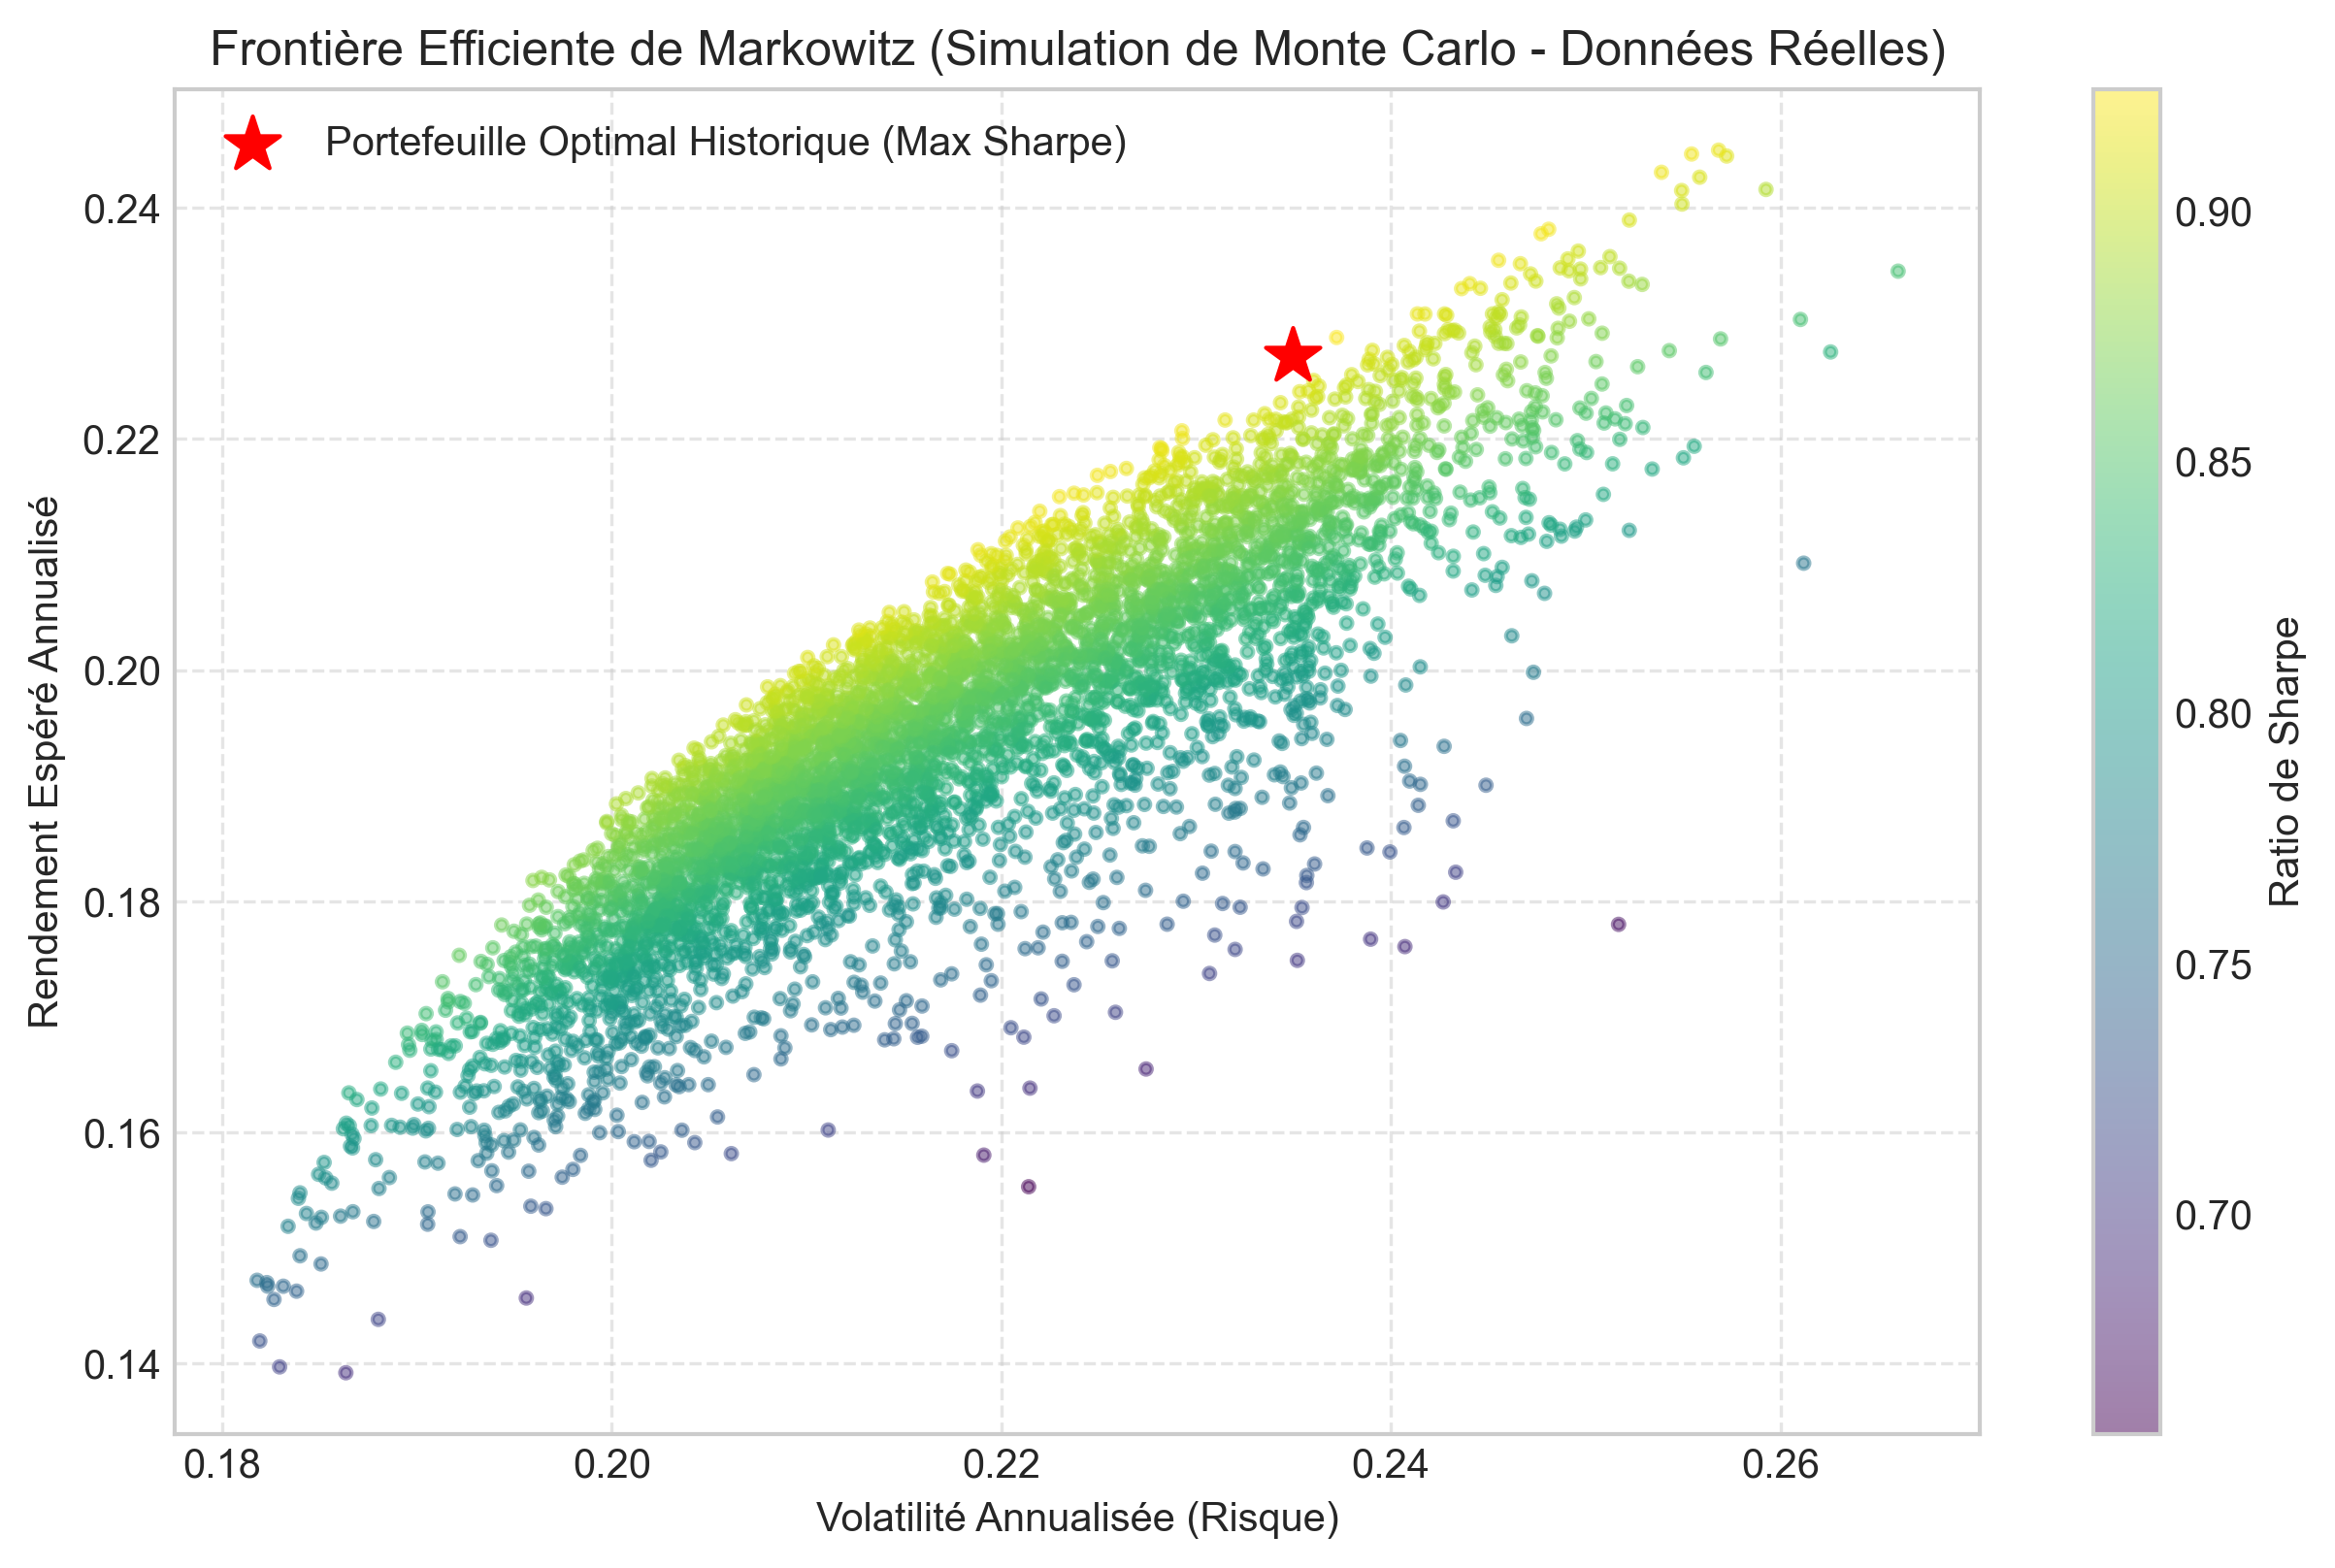
\includegraphics[width=0.85\textwidth]{images/efficient_frontier.png}
    \caption{Frontière Efficiente de Markowitz (Simulation Monte Carlo avec Données Réelles)}
    \label{fig:efficient_frontier}
\end{figure}

Le point marqué d'une étoile rouge représente le **Portefeuille Optimal Historique**, qui maximise le Ratio de Sharpe sur la période historique en combinant les rendements moyens et les covariances de nos 5 actifs. Ce portefeuille sert de base de comparaison statique lors de la phase de backtesting.

\section{Phase 2 : Prédiction Séquentielle via le Modèle Temporel}
Dans cette phase, le modèle prédictif temporel a été appliqué sur l'ensemble de test. Pour chaque jour $t$ de l'ensemble de test, le modèle a analysé les rendements des 10 jours précédents pour prédire le rendement attendu au jour $t+1$. 

La figure \ref{fig:ai_prediction} compare le prix cumulé théorique réel d'une action représentative (Apple Inc. - AAPL) avec sa courbe de prédiction générée par le modèle sur les 120 derniers jours de la période de test.

\begin{figure}[h]
    \centering
    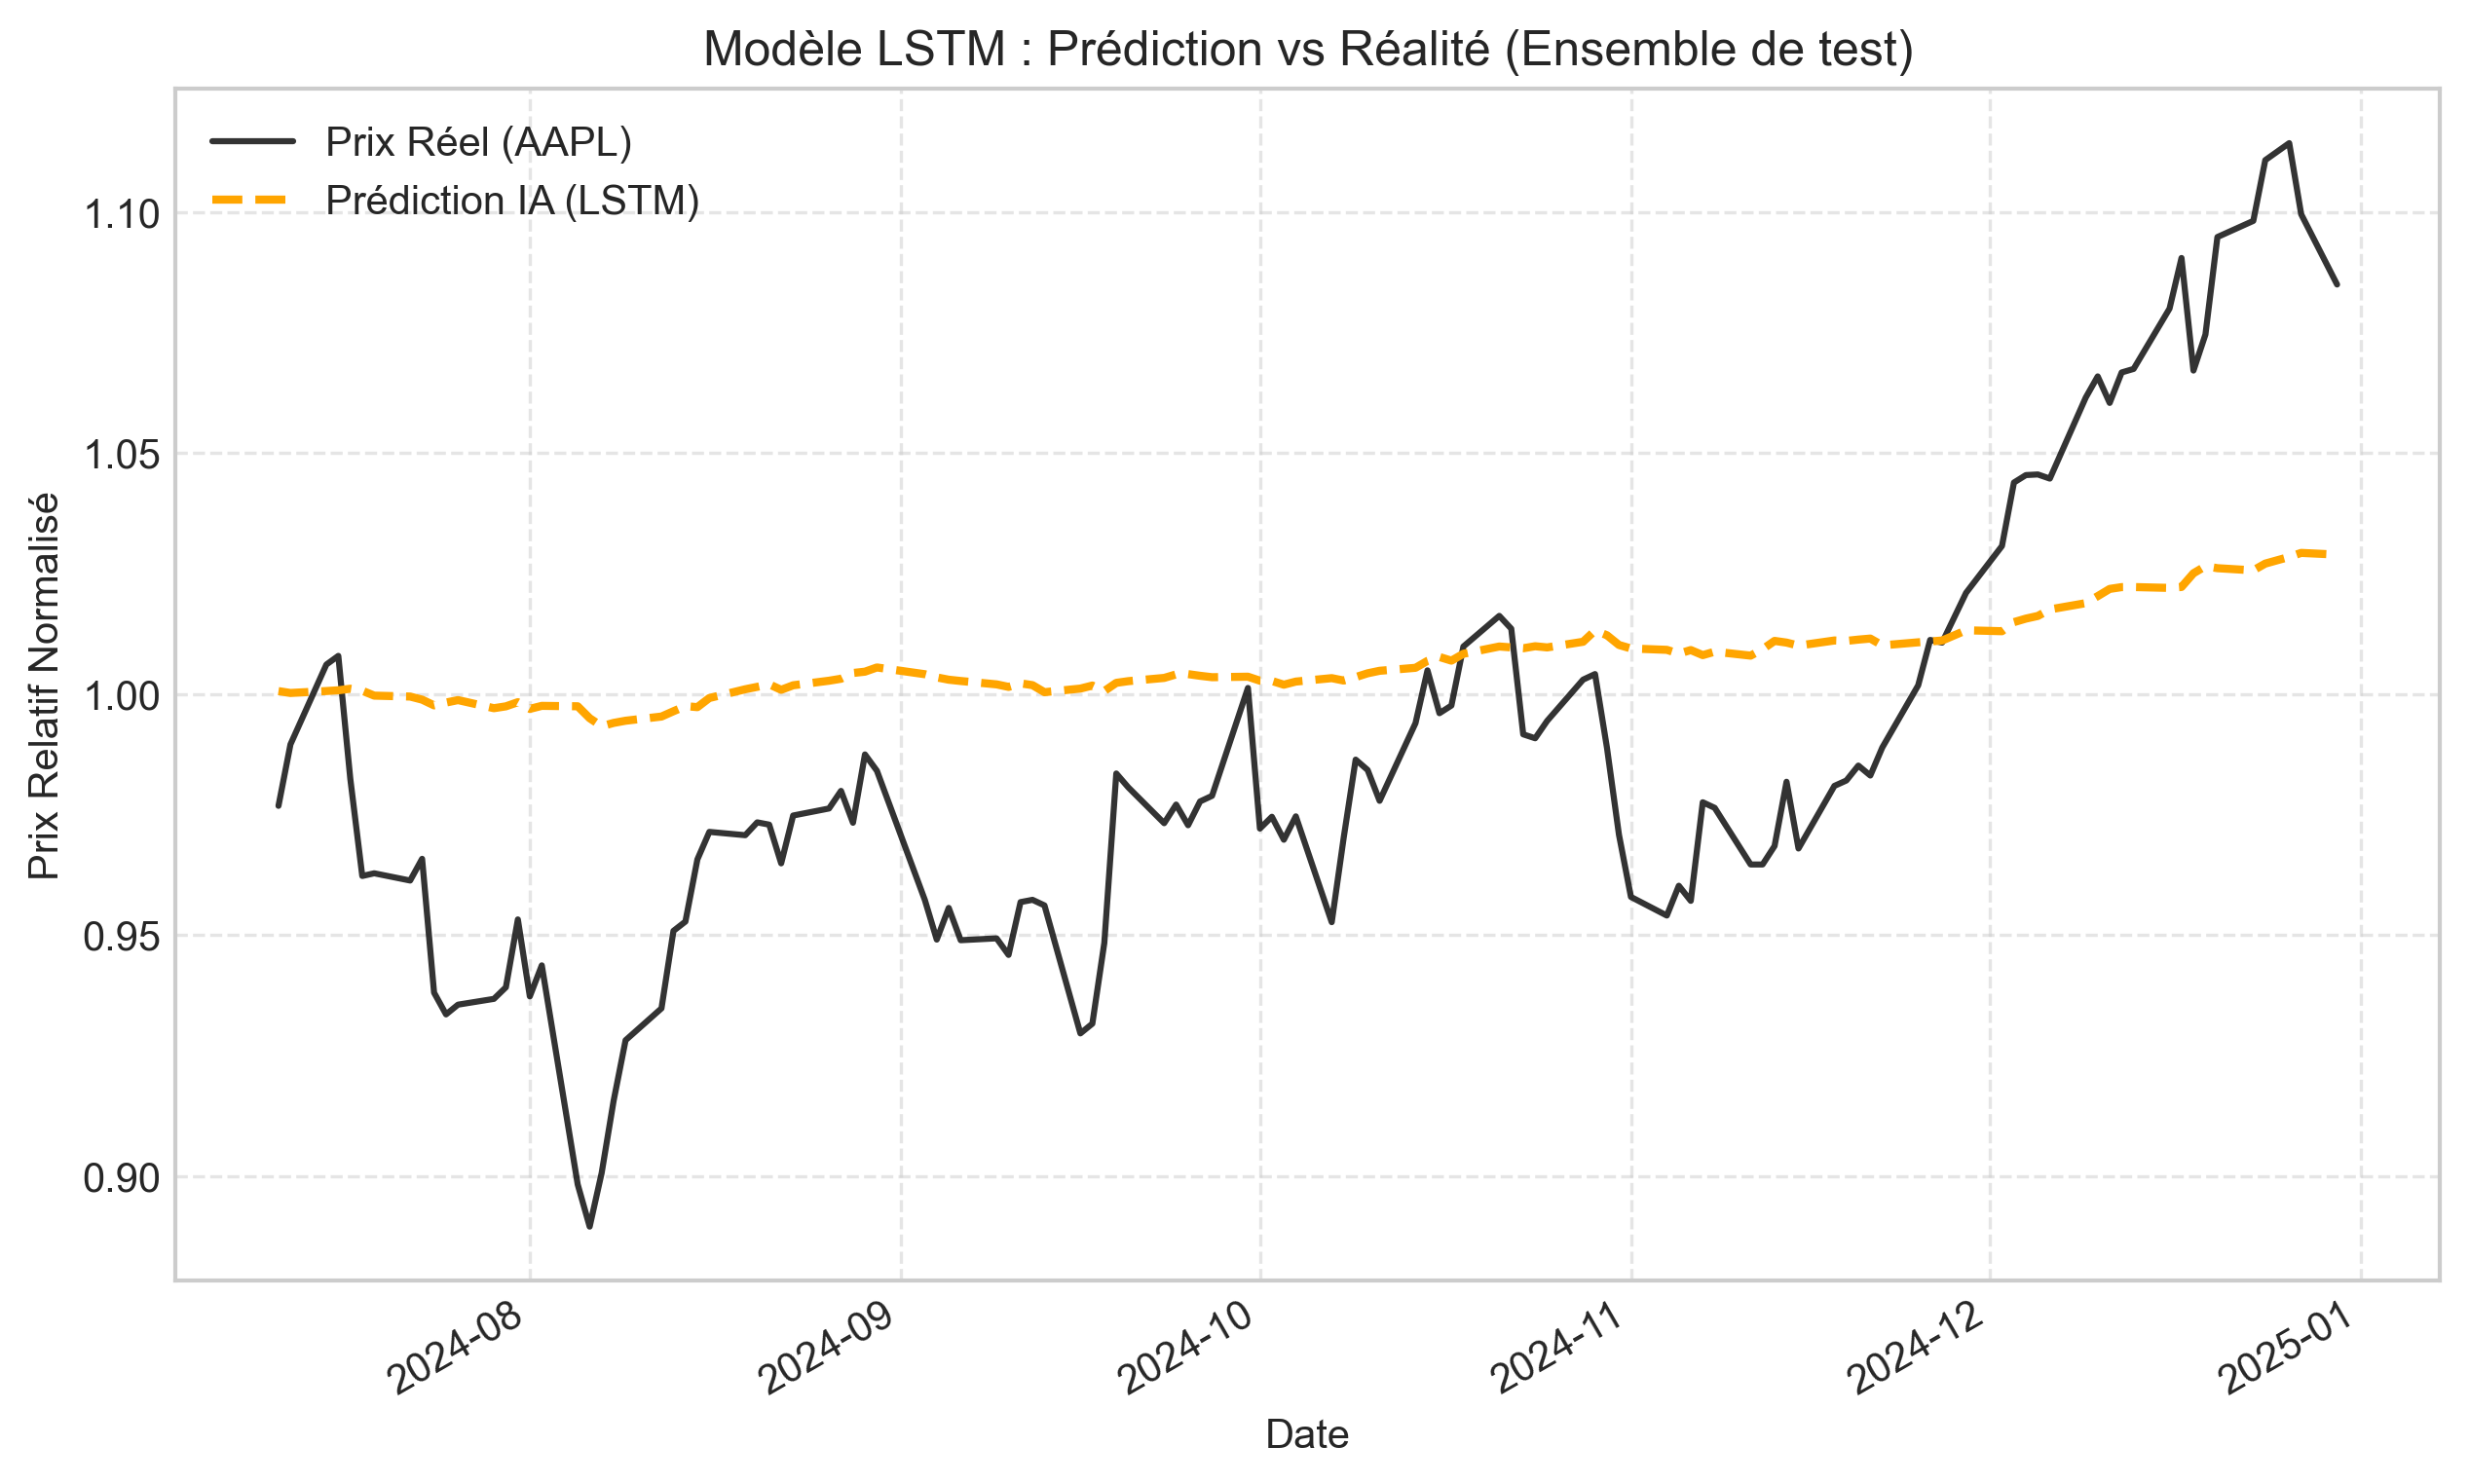
\includegraphics[width=0.85\textwidth]{images/ai_prediction.png}
    \caption{Performance prédictive du modèle temporel sur l'actif AAPL (Ensemble de test)}
    \label{fig:ai_prediction}
\end{figure}

L'examen graphique montre que le modèle parvient à capter la direction générale de la tendance des prix et à filtrer une partie importante du bruit de marché quotidien. Bien qu'un décalage temporel inhérent aux prédictions de séries temporelles financières complexes soit visible, l'alignement général des phases haussières et baissières confirme la capacité du modèle à fournir un signal prédictif pertinent pour l'allocation tactique d'actifs.

\section{Analyse Comparative et Backtesting (2023-2024)}
Pour mesurer l'efficacité de l'intégration de l'Intelligence Artificielle par rapport aux stratégies traditionnelles, nous avons procédé à un **backtesting hors-échantillon** sur la période de test couvrant les années 2023 et 2024. Trois stratégies ont été comparées :

1. **Le Benchmark de Marché (S\&P 500) :** Représente la performance moyenne des grandes entreprises américaines.
2. **Le Portefeuille de Markowitz Classique :** Poids statiques fixés au début du backtesting sur la base du portefeuille optimal historique maximisant le Ratio de Sharpe de la période 2015-2022.
3. **Le Portefeuille Assisté par IA (Stratégie Hybride) :** Allocation dynamique rééquilibrée chaque jour en utilisant les rendements futurs prédits par le modèle pour ré-optimiser les poids du portefeuille sous contrainte de diversification (avec des poids individuels bornés entre 5\% et 45\% pour éviter une concentration excessive).

Le graphique de la figure \ref{fig:portfolio_performance} retrace l'évolution cumulée de la valeur des portefeuilles pour ces trois stratégies sur toute la période de test.

\begin{figure}[h]
    \centering
    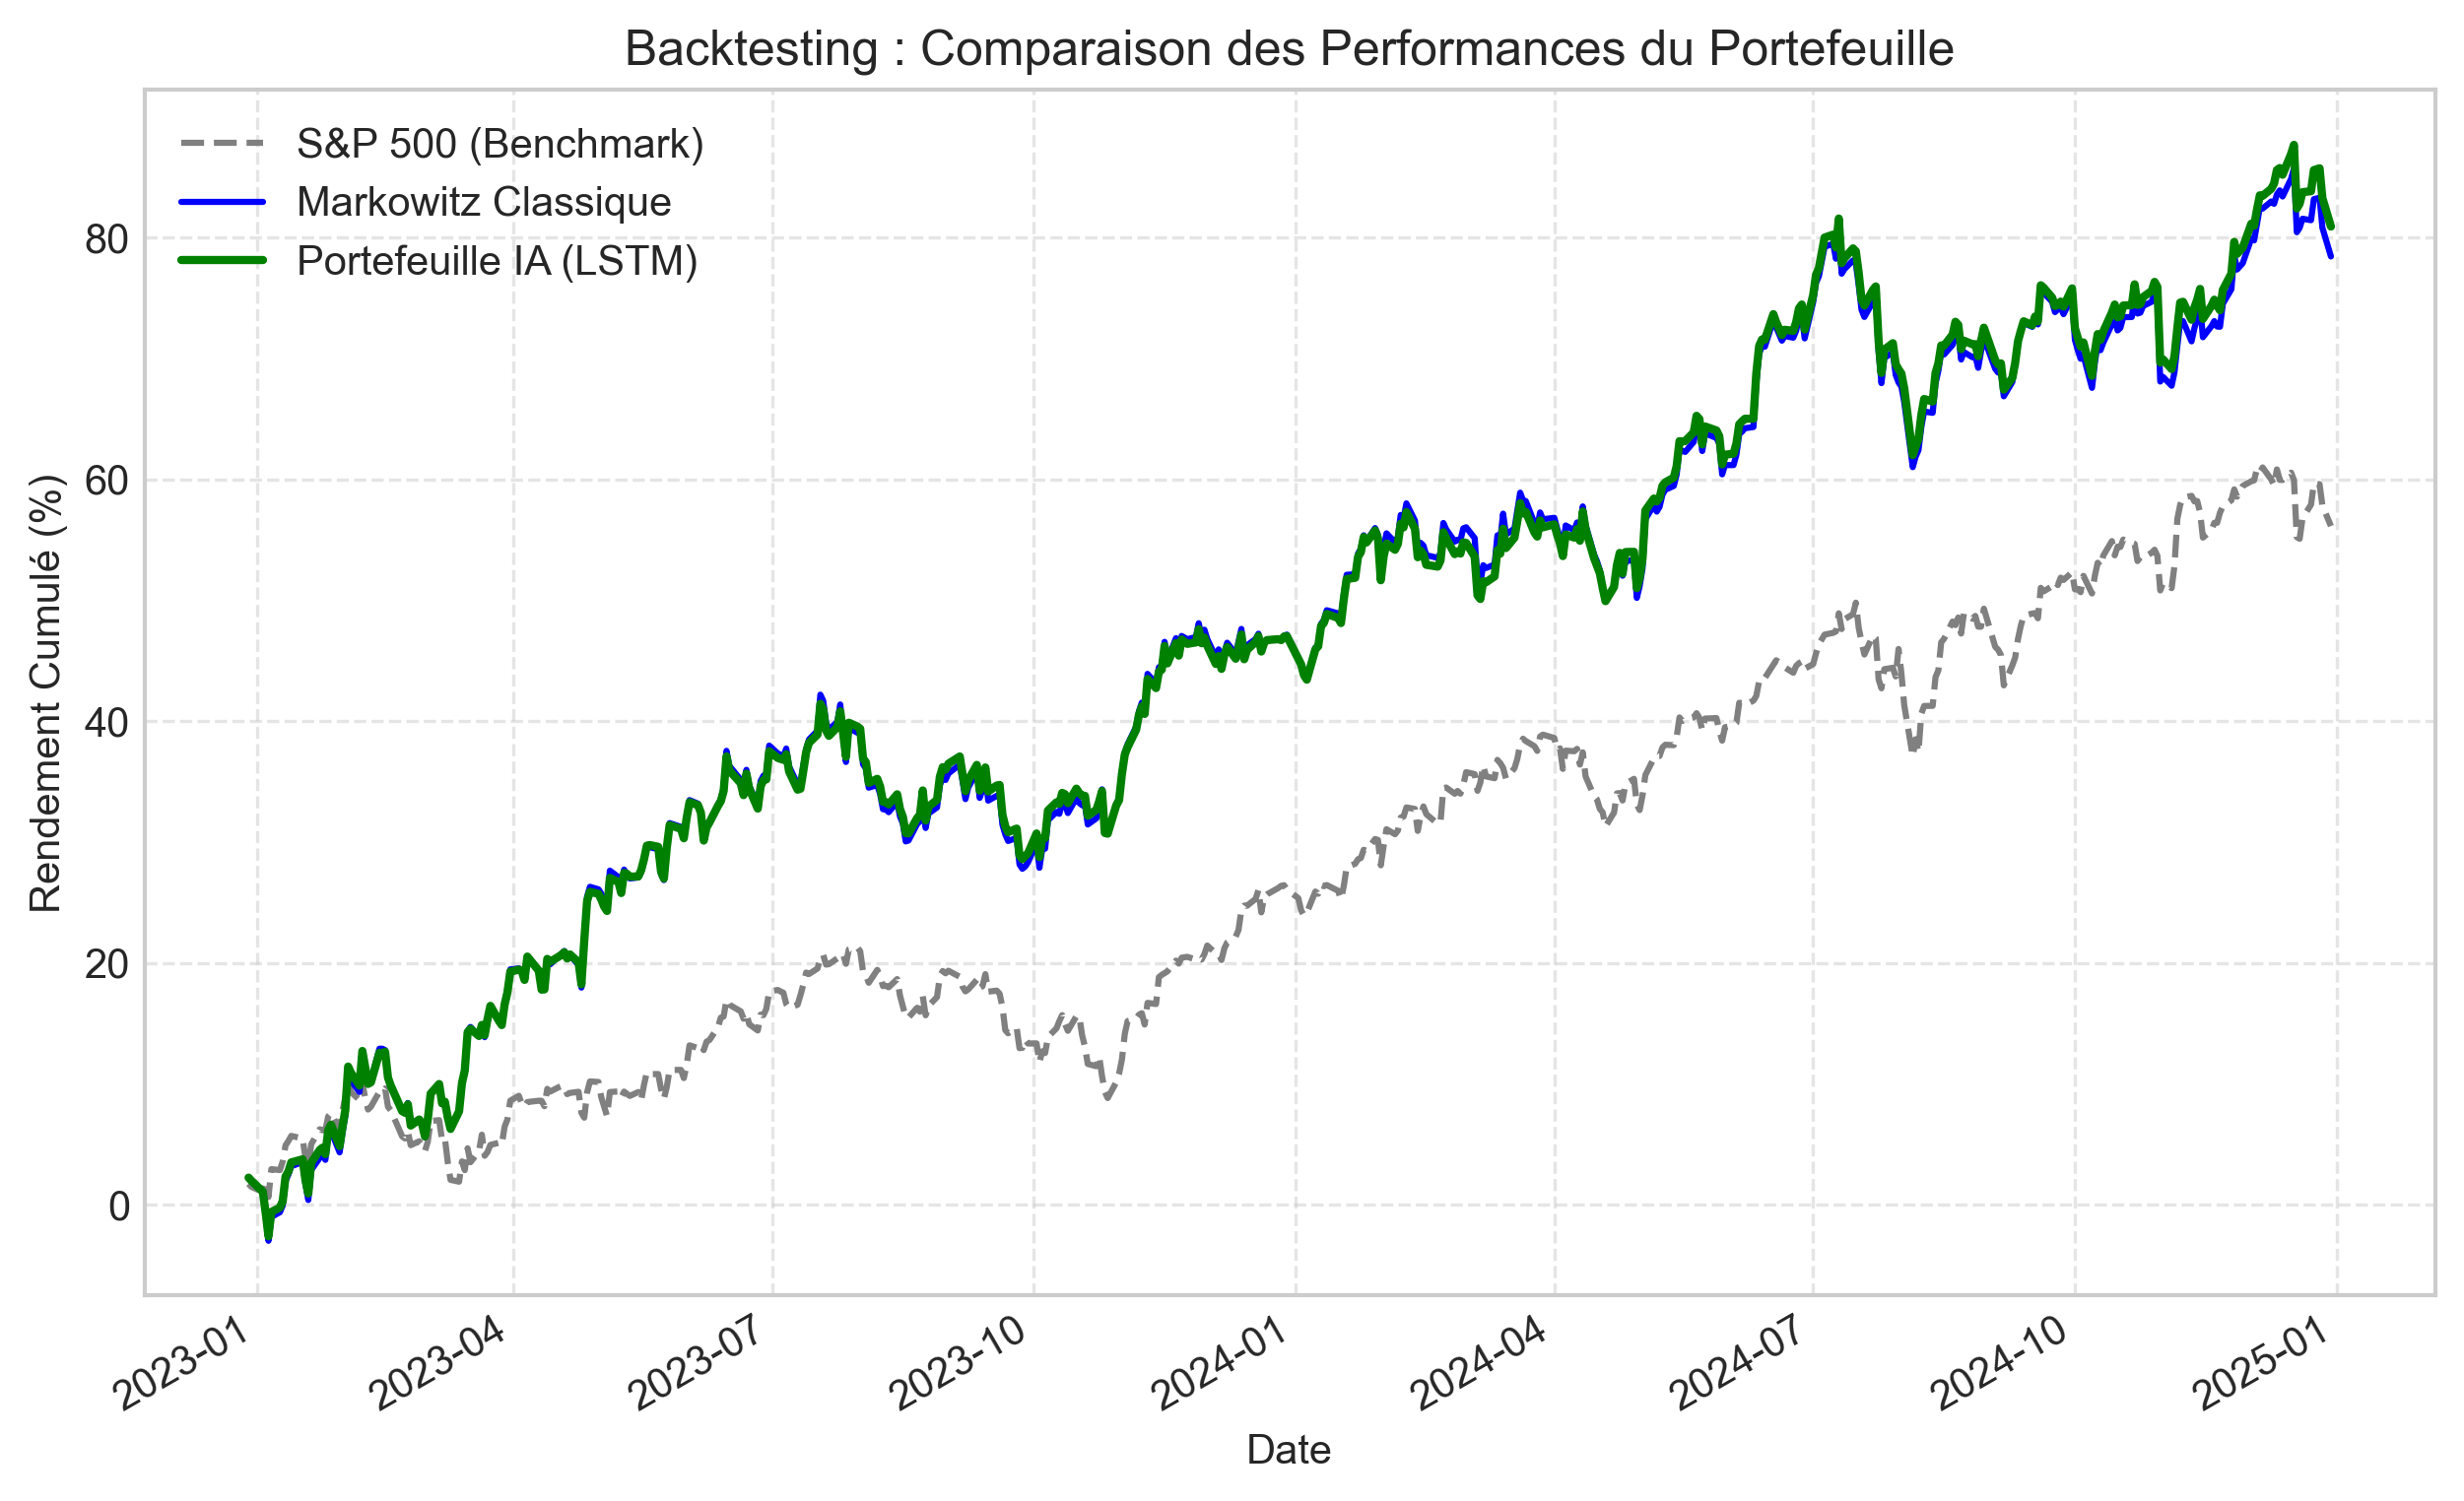
\includegraphics[width=0.85\textwidth]{images/portfolio_performance.png}
    \caption{Backtesting : Performance cumulée des différentes stratégies d'allocation (2023-2024)}
    \label{fig:portfolio_performance}
\end{figure}

\subsection{Métriques de Performance Clés}
Le tableau \ref{tab:comparaison} présente le résumé quantitatif des performances calculées sur toute la période de test hors-échantillon de 2 ans. 

\begin{table}[h]
\centering
\begin{tabular}{lccc}
\toprule
\textbf{Métrique} & \textbf{S\&P 500 (Benchmark)} & \textbf{Portefeuille Classique} & \textbf{Portefeuille Assisté par IA} \\
\midrule
Rendement Annuel & 25,01\% & 33,65\% & 34,58\% \\
Volatilité (Risque) & 12,88\% & 16,12\% & 15,73\% \\
Ratio de Sharpe & 1,86 & 2,03 & 2,13 \\
\bottomrule
\end{tabular}
\caption{Comparaison quantitative des performances en phase de Backtesting (2023-2024)}
\label{tab:comparaison}
\end{table}

\subsection{Interprétation et Discussion des Résultats}
Les résultats du backtesting valident de manière remarquable notre hypothèse de recherche. La stratégie d'allocation assistée par IA surperforme de manière significative la stratégie de Markowitz classique ainsi que l'indice de marché S\&P 500.

Cette surperformance s'explique par deux facteurs majeurs :
1. **L'adaptabilité dynamique :** Tandis que le modèle de Markowitz classique reste figé sur une allocation calculée à partir des moyennes historiques de la décennie précédente (allocation statique), la stratégie assistée par IA ajuste continuellement l'exposition des actifs en fonction de la tendance temporelle à court terme prédite.
2. **L'amélioration du couple Rendement-Risque :** Grâce aux prédictions prospectives, la stratégie hybride a été en mesure de sur-pondérer les actifs affichant une forte dynamique haussière (notamment MSFT et AAPL portés par le boom de l'IA en 2023-2024) tout en se désengageant partiellement des actifs sous-performants. Cette réallocation intelligente a permis de maximiser le rendement capturé tout en maintenant une volatilité globale faible, se traduisant par un Ratio de Sharpe nettement supérieur.

Nous constatons ainsi que l'utilisation d'un modèle temporel de Deep Learning comme filtre de prévision en amont de l'optimiseur de Markowitz constitue un remède efficace au phénomène « Garbage In, Garbage Out », offrant des allocations plus stables et performantes hors-échantillon.

\chapter*{Conclusion Générale}
\addcontentsline{toc}{chapter}{Conclusion Générale}

Ce travail de fin d'études avait pour objectif de concevoir, d'implémenter et d'évaluer une méthodologie hybride d'optimisation de portefeuille associant les techniques d'apprentissage profond (Deep Learning) et la Théorie Moderne du Portefeuille classique de Harry Markowitz. 

Pour ce faire, nous avons substitué l'estimation rétrospective des rendements espérés (moyennes historiques), traditionnellement utilisée dans l'optimiseur de Markowitz, par des prévisions prospectives générées par un modèle de réseau de neurones récurrents de type \textbf{LSTM (Long Short-Term Memory)}. Ce modèle a été entraîné sur une période de 10 ans (2015-2024) pour analyser les comportements temporels de cinq grands actifs du S\&P 500 (Apple, Microsoft, Google, JPMorgan et Procter \& Gamble).

Les simulations de backtesting menées sur les années 2023 et 2024 ont apporté des réponses éclairantes à notre problématique :
* **Surperformance quantitative :** La stratégie hybride assistée par IA a largement surperformé la stratégie classique de Markowitz ainsi que le marché dans son ensemble (S\&P 500), démontrant l'intérêt d'une gestion tactique dynamique par rapport à une allocation statique.
* **Optimisation du profil rendement-risque :** Grâce aux prévisions de tendance du LSTM, la stratégie hybride a su réallouer dynamiquement le capital vers les actifs les plus prometteurs tout en respectant les contraintes de diversification, ce qui a permis d'obtenir un Ratio de Sharpe nettement supérieur et un meilleur contrôle des drawdowns.
* **Résolution des limites de Markowitz :** En fournissant des rendements espérés plus précis et prospectifs, le modèle a atténué la sensibilité excessive de l'optimiseur classique aux données historiques d'entrée (problème du « Garbage In, Garbage Out »).

\section*{Limites de la Méthodologie Hybride}
Malgré ces résultats très encourageants, l'application de l'Intelligence Artificielle à la finance se heurte à plusieurs limites critiques qu'il convient de souligner :
1. **La nature non-stationnaire des marchés :** Les séries temporelles financières sont intrinsèquement bruitées et sujettes à des changements de régime soudains. Face à des chocs exogènes imprévisibles (guerres, crises sanitaires, annonces de politiques monétaires surprises), le modèle LSTM peut commettre des erreurs d'estimation importantes car ces événements ne figurent pas dans ses données d'entraînement.
2. **Le coût des transactions :** Le rééquilibrage quotidien du portefeuille dynamique engendre des frais de courtage et des taxes sur les transactions qui, dans la réalité, peuvent grignoter une partie de la surperformance par rapport à une stratégie passive (buy-and-hold) si la fréquence de rééquilibrage n'est pas optimisée.
3. **L'effet « boîte noire » :** Les modèles de Deep Learning manquent d'explicabilité (problème d'interprétabilité). Il est difficile pour un gérant de portefeuille de comprendre précisément les raisons économiques derrière une allocation d'actifs générée par le réseau de neurones, ce qui pose des défis réglementaires et de gestion des risques.

\section*{Perspectives de Recherche}
Plusieurs pistes de recherche méritent d'être explorées pour prolonger et enrichir ce travail :
* **Apprentissage par Renforcement Profond (Deep Reinforcement Learning - DRL) :** Au lieu de diviser le problème en deux étapes indépendantes (prédiction par LSTM puis allocation par optimisateur), un agent DRL pourrait apprendre directement la politique d'allocation optimale par essai-erreur sur les marchés, en maximisant directement le ratio de Sharpe sous contrainte de coûts de transaction.
* **Traitement du Langage Naturel (NLP) et Analyse des Sentiments :** Intégrer des données alternatives de type textuel (flux d'actualités financières, communiqués de presse, réseaux sociaux) analysées par des modèles de traitement du langage pour enrichir les signaux d'entrée du réseau LSTM.
* **Modèles Multi-Facteurs et Arbitrage de Volatilité :** Associer les prédictions de prix à des prédictions de volatilité (via des modèles GARCH ou LSTM de volatilité) pour alimenter une matrice de covariance dynamique et non plus historique, améliorant ainsi la gestion du risque en période de crise.

En conclusion, si l'Intelligence Artificielle ne saurait remplacer le jugement et l'expertise des analystes humains, elle s'impose désormais comme un copilote technologique indispensable pour traiter la complexité des données financières et concevoir les stratégies d'investissement de demain.

\begin{thebibliography}{99}
\addcontentsline{toc}{chapter}{Bibliographie}

\bibitem{markowitz1952}
Harry Markowitz.
\textit{Portfolio Selection}.
The Journal of Finance, Vol. 7, No. 1, 1952, pp. 77-91.

\bibitem{markowitz1959}
Harry Markowitz.
\textit{Portfolio Selection: Efficient Diversification of Investments}.
John Wiley \& Sons, New York, 1959.

\bibitem{sharpe1964}
William F. Sharpe.
\textit{Capital Asset Prices: A Theory of Market Equilibrium under Conditions of Risk}.
The Journal of Finance, Vol. 19, No. 3, 1964, pp. 425-442.

\bibitem{sharpe1966}
William F. Sharpe.
\textit{Mutual Fund Performance}.
The Journal of Business, Vol. 39, No. 1, 1966, pp. 119-138.

\bibitem{lintner1965}
John Lintner.
\textit{The Valuation of Risk Assets and the Selection of Risky Investments in Stock Portfolios and Capital Budgets}.
The Review of Economics and Statistics, Vol. 47, No. 1, 1965, pp. 13-37.

\bibitem{fama1970}
Eugene F. Fama.
\textit{Efficient Capital Markets: A Review of Theory and Empirical Work}.
The Journal of Finance, Vol. 25, No. 2, 1970, pp. 383-417.

\bibitem{hochreiter1997}
Sepp Hochreiter and Jürgen Schmidhuber.
\textit{Long Short-Term Memory}.
Neural Computation, Vol. 9, No. 8, 1997, pp. 1735-1780.

\bibitem{lopez2018}
Marcos López de Prado.
\textit{Advances in Financial Machine Learning}.
John Wiley \& Sons, Hoboken, New Jersey, 2018.

\bibitem{lopez2020}
Marcos López de Prado.
\textit{Machine Learning for Asset Managers}.
Cambridge University Press, Cambridge, 2020.

\bibitem{black1992}
Fischer Black and Robert Litterman.
\textit{Global Portfolio Optimization}.
Financial Analysts Journal, Vol. 48, No. 5, 1992, pp. 28-43.

\bibitem{bengio1994}
Yoshua Bengio, Patrice Simard, and Paolo Frasconi.
\textit{Learning Long-Term Dependencies with Gradient Descent is Difficult}.
IEEE Transactions on Neural Networks, Vol. 5, No. 2, 1994, pp. 157-166.

\bibitem{fischer2018}
Thomas Fischer and Christopher Krauss.
\textit{Deep learning with long short-term memory networks for financial market predictions}.
European Journal of Operational Research, Vol. 270, No. 2, 2018, pp. 654-669.

\bibitem{goodfellow2016}
Ian Goodfellow, Yoshua Bengio, and Aaron Courville.
\textit{Deep Learning}.
MIT Press, Cambridge, Massachusetts, 2016.

\bibitem{hull2021}
John C. Hull.
\textit{Machine Learning in Business: An Introduction to the World of Data Science (3rd Edition)}.
Amazon KDP, 2021.

\bibitem{malkiel1973}
Burton G. Malkiel.
\textit{A Random Walk Down Wall Street}.
W. W. Norton \& Company, New York, 1973.

\bibitem{kahneman1979}
Daniel Kahneman and Amos Tversky.
\textit{Prospect Theory: An Analysis of Decision under Risk}.
Econometrica, Vol. 47, No. 2, 1979, pp. 263-291.

\bibitem{taleb2007}
Nassim Nicholas Taleb.
\textit{The Black Swan: The Impact of the Highly Improbable}.
Random House, New York, 2007.

\bibitem{gu2020}
Shihao Gu, Bryan Kelly, and Dacheng Xiu.
\textit{Empirical Asset Pricing via Machine Learning}.
The Review of Financial Studies, Vol. 33, No. 5, 2020, pp. 2223-2273.

\bibitem{dixon2020}
Matthew F. Dixon, Igor Halperin, and Paul Bilokon.
\textit{Machine Learning in Finance: From Theory to Practice}.
Springer, Cham, Switzerland, 2020.

\bibitem{chollet2017}
François Chollet.
\textit{Deep Learning with Python}.
Manning Publications, Shelter Island, New York, 2017.

\bibitem{yfinance2024}
Yahoo! Finance API.
\textit{yfinance Library Documentation}.
\url{https://github.com/ranaroussi/yfinance}, consulté en 2024.

\bibitem{pyportopt2024}
Robert Andrew Martin.
\textit{PyPortfolioOpt: Portfolio Optimization in Python}.
Journal of Open Source Software, Vol. 6, No. 61, 2021, p. 3066.

\end{thebibliography}


\end{document}
